%!TEX root=../../main.tex
\section{Frontend}
\label{chapter:implementierung-frontend}
In diesem Kapitel wird die Implementierung des Frontends von \textit{Refundable} erläutert. Dabei wird als Erstes die Vorbereitung im \autoref{chapter:implementierung-frontend-vorbereitung} erklärt. Danach werden die einzelnen Komponenten im \autoref{chapter:implementierung-frontend-komponenten} der Website erklärt und vorgeführt.
\subsection{Vorbereitung}
\label{chapter:implementierung-frontend-vorbereitung}
Wie im \autoref{chapter:study-frontend} und \autoref{chapter:study-datenschnittstelle} festgelegt wird im Frontend Bootstrap in Verbindung mit VueJS verwendet. Zu aller erst muss daher VueJS auf dem Computer, auf dem das Projekt erstellt wird, installiert werden. Dies geschieht auf Windows über den Node Packet Manager (NPM) \cite{vue-install}. Der Befehl um VueJS zu installieren schaut wie folgt aus:
\begin{code}{bash}
	npm install -g @vue/cli
\end{code}
Nachdem VueJS installiert ist kann man in das gewünschte Verzeichnis wechseln und über
\begin{code}{bash}
	vue create refundable
\end{code}
ein neues Vue Projekt erstellen, das in diesem Fall \textit{Refundable} heißt \cite{vue-create-project}. Um die Funktionalität von Bootstrap und VueJS optimal auszunutzen, wird Bootstrap direkt mit dem Node Packet Manager zu VueJS installiert \cite{bootstrap-vue-getting-started}:
\begin{code}{bash}
	npm install vue bootstrap-vue
\end{code}
Um in den Komponenten Bootstrap und dessen vordefinierte Icons zu verwenden, muss man in \enquote{main.js} folgendes importieren:
\begin{code}{html}
	import { BootstrapVue, BootstrapVueIcons } from "bootstrap-vue";
	import "./plugins/bootstrap-vue";
	
	Vue.use(BootstrapVue);
	Vue.use(BootstrapVueIcons);
\end{code}
\captionof{listing}{Benötigte Befehle um Bootstrap im VueJS Projekt einzubinden}
	\label{list:requcommands} ~\\
Alle Teile der Website sind in sogenannten Komponenten verpackt, die je nach Benutzereingaben dynamisch gewechselt werden. 

\newpage
\subsection{Komponenten der Website}
\label{chapter:implementierung-frontend-komponenten}
\subsubsection{Generell}
\label{chapter:implementierung-frontend-komponenten-generell}
Die Struktur der Komponenten ist so aufgebaut, dass die Seite sowohl für Desktop- als auch mobile Endgeräte optimiert ist. Dazu wird das \enquote{Grid-System} von Bootstrap verwendet, welches seinen Platz im \enquote{template-Tag}, der VueJS Komponente findet. Dieses besteht aus einem Container, einer Reihe (Row) und einer Spalte (Column). Da es am Anfang das Problem gab, dass nicht der ganze Bildschirm ausgenutzt wird, wurden folgende Klassen im CSS-Dokument erstellt:
\begin{code}{css}
	.template-main-container {
		height: 100vh;
		width: 100vw;
		margin: 0;
		padding: 0;
	}
	
	.template-main-row {
		height: 100vh;
		width: 100vw;
		margin: 0;
		padding: 0;
	}
\end{code}
\captionof{listing}{CSS Klassen für die Haupt- Contianer und Reihen}
	\label{list:cssmaincont} ~\\
Diese dienen dazu, dass der Hauptcontainer, als auch die Hauptreihe der Website, 100\% der Höhe (100 vertikale Einheiten), sowie 100\% der Breite (100 horizontale Einheiten) einnehmen. Außerdem wird in den Klassen definiert, dass die Elemente keinen Abstand zum Rand, der Seite haben sollen.
\newpage
\subsubsection{Login-Seite}
\label{chapter:implementierung-frontend-komponenten-login}
Die Login-Seite sollte sehr schlicht gehalten werden und sofort verstamden werden können. Da das Tool \textit{Refundable} nur von Lehrern des TGMs verwendet werden soll, wurde in der Loginmaske die E-Mail-Endung \enquote{@tgm.ac.at} vordefiniert. Außerdem soll dem Aufrufer der Website sofort klar machen, worum es sich bei dieser Website handelt und haben daher den Projektnamen \textit{Refundable}, als auch unseren Slogan auf der Seite platziert. Des weiteren war aufgrund der DSGVO eine Meldung zu realisieren, die den Benutzer darüber informiert, dass Cookies verwendet werden. Falls diese Meldung nicht akzeptiert wird und man sich anzumelden möchte, wird eine Fehlermeldung dargestellt. Diese Meldung wird jedoch dynamisch mit VueJS erstellt und nicht direkt mittels Bootstrap. In der Umsetzung schaut die Login-Seite wie folgt aus (\autoref{fig:login}):
\begin{figure}[H]
	\centering
	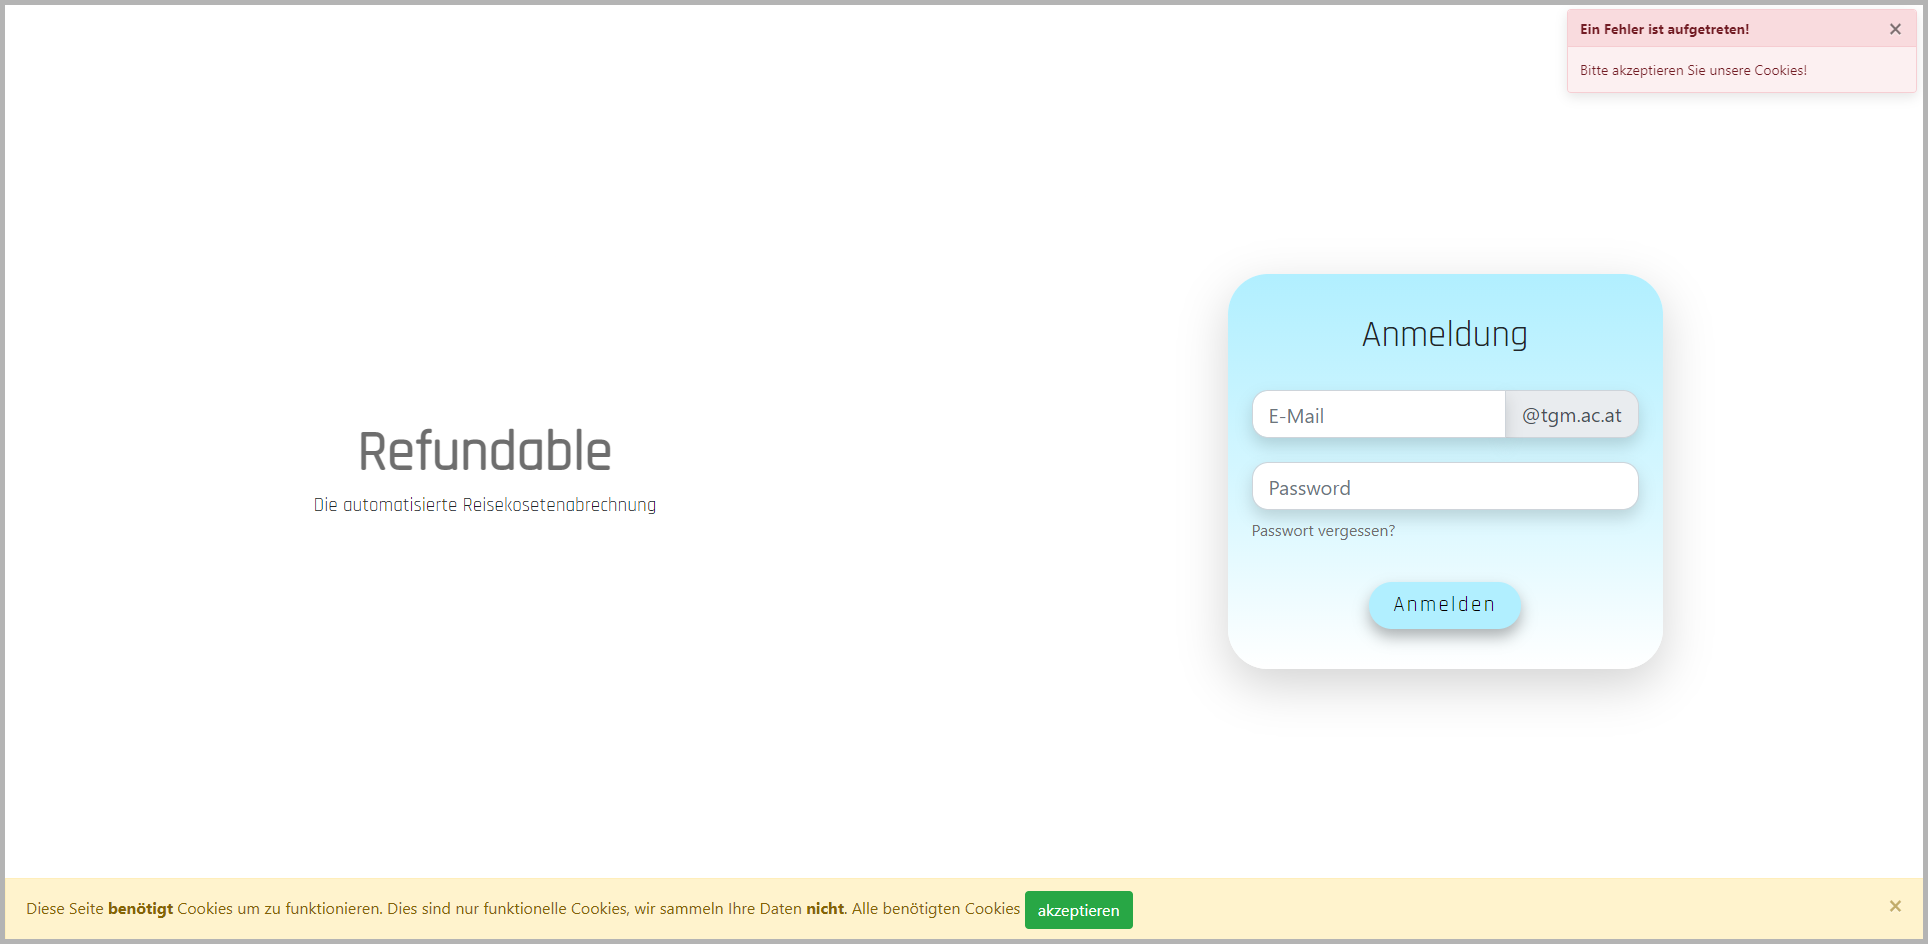
\includegraphics[width=1\linewidth]{images/website/login}
	\caption[Login]{Ein Bild der Login-Seite}
	\label{fig:login}
\end{figure}
\paragraph{Login-Maske}
~\\
Die Login-Maske besteht aus einem eigenen Container, welcher ermöglicht die Maske vollkommen responsiv aufzubauen. Die Eingabefelder wurden mit einer \enquote{input-groupe} gelößt (Code Z. 12). Um einen Wert optisch in einem Eingabefeld, vorzugeben hat Bootstrap ein Element, namens \enquote{b-input-groupe-text} (Code Z. 14), welches vor oder nach dem Feld hinzugefügt werden kann. Da die Login-Daten, der TGM Server verwendet werden, haben wir einen Link eingebaut, falls man sein Passwort vergessen hat. Betätigt man diesen, wird man auf die entsprechende Seite des TGMs weitergeleitet.
\begin{code}{html}
	<!-- Anmeldungsformular -->
	<b-col cols="12" md="6">
		<b-container>
			<b-row align-h="center">
				<b-col cols="12" sm="10" md="10" lg="8" xl="6">
					<b-container id="login-wrap" class="shadow-lg">
						<b-row id="r-login" align-h="center">
							<h2 id="lheading2">Anmeldung</h2>
						</b-row>
						<b-row align-h="center" id="r-email">
							<b-col cols="12">
								<!-- Input des Benutzernamens / der Email -->
								<b-input-group size="lg">
									<b-input-group-text
										id="tgm-addon"
										class="shadow"
										slot="append"
										><span>@tgm.ac.at</span></b-input-group-text
										>
									<b-form-input
										id="email"
										class="shadow login-inputs"
										v-model="email"
										type="text"
										placeholder="E-Mail"
									></b-form-input>
								</b-input-group>
							</b-col>
						</b-row>
						<b-row id="r-password">
							<b-col cols="12">
								<!-- Input des Passworts -->
								<b-form-input
									id="password"
									class="shadow login-inputs"
									v-model="password"
									type="password"
									placeholder="Password"
									size="lg"
								></b-form-input>
							</b-col>
						</b-row>
						<b-row id="r-forgotten">
							<b-col cols="12">
								<!-- Passwort vergessen Weiterleitung auf Moodle -->
								<a
									id="forgotten-password"
									href="https://elearning.tgm.ac.at/login/forgot_password.php"
								>Passwort vergessen?</a
								>
							</b-col>
						</b-row>
						<b-row align-h="center" id="r-login-btn">
							<!-- Login Button -->
							<b-button size="lg" id="login-btn" v-on:click="login"
							>Anmelden</b-button
							>
						</b-row>
					</b-container>
				</b-col>
			</b-row>
		</b-container>
	</b-col>
\end{code}
\captionof{listing}{HTML Code der Login-Maske}
	\label{list:loginmask} ~\\
Da einige Elemente unseren Ansprüchen optisch nicht genügt haben, wurden eigene Änderungen im CSS-Code hinzugefügt. Dabei wurde vor allem die Gestaltung, der Eingabefelder und des Buttons verändert, aber auch jene des Containers, welcher die Maske beinhaltet. Es wurde der Farbverlauf des Logos in der Maske eingebaut und die Ecken der Elemente etwas abgerundet.
\begin{code}{css}
/* -- Login -- */

#login-wrap {
	background: rgb(255, 255, 255);
	background: -moz-linear-gradient(
	0deg,
	rgba(255, 255, 255, 1) 0%,
	rgba(220, 248, 255, 1) 38%,
	rgba(177, 239, 255, 1) 100%
	);
	background: -webkit-linear-gradient(
	0deg,
	rgba(255, 255, 255, 1) 0%,
	rgba(220, 248, 255, 1) 38%,
	rgba(177, 239, 255, 1) 100%
	);
	background: linear-gradient(
	0deg,
	rgba(255, 255, 255, 1) 0%,
	rgba(220, 248, 255, 1) 38%,
	rgba(177, 239, 255, 1) 100%
	);
	filter: progid: DXImageTransform.Microsoft.gradient(startColorstr="#ffffff", endColorstr="#b1efff", GradientType=1);
	padding: 1.5rem;
	border-radius: 2.5rem;
}

#email {
	border-radius: 1rem 0 0 1rem;
}

#tgm-addon {
	border-radius: 0 1rem 1rem 0;
}

.input-group-append {
	border-radius: 0 1rem 1rem 0;
}

.input-group-text {
	border-radius: 0 1rem 1rem 0;
}

#password {
	border-radius: 1rem 1rem 1rem 1rem;
}

#login-btn {
	font-family: "Rajdhani", sans-serif;
	padding: 0.5rem 1.5rem 0.5rem 1.5rem;
	font-size: 1.3rem;
	letter-spacing: 2.5px;
	font-weight: 500;
	color: #000;
	background-color: rgba(177, 239, 255, 1);
	border: none;
	border-radius: 45px;
	box-shadow: 0px 8px 15px rgba(0, 0, 0, 0.3);
	transition: all 0.3s ease 0s;
	cursor: pointer;
	outline: none;
}

#login-btn:hover {
	background-color: #2ec0e5;
	box-shadow: 0px 15px 20px rgba(46, 229, 157, 0);
	color: #fff;
	transform: translateY(3px);
}
\end{code}
\captionof{listing}{CSS Code der Login-Maske}
	\label{list:csslogin} ~\\
\paragraph{Cookie-Meldung}
~\\
Die Meldung, dass Cookies benutzt werden, sollte schlicht und einfach sein. Es wurden die Anforderungen an die Meldung gestellt, dass sie dem Nutzer informieren soll, dass ausschließlich funktionelle und notwendige Cookies verwendet werden. Für diese Meldung hat sich perfekt das vordefinierte \enquote{Alert-Element} von Bootstrap geeignet:
\makeatletter
\begin{code}{html}
	<!-- Bestätigung, dass diese Seite Cookies benutzt -->
	<b-alert
		v-model="showBottom"
		class="position-fixed fixed-bottom m-0 rounded-0"
		style="z-index: 2000;"
		variant="warning"
		dismissible
	>
		Diese Seite <b>benötigt</b> Cookies um zu funktionieren. Dies sind nur
		funktionelle Cookies, wir sammeln Ihre Daten <b>nicht</b>. Alle benötigten
		Cookies
		<!-- Button zum akzeptieren -->
		<b-button variant="success" @click="validateCookies()"
			>akzeptieren
		</b-button>
	</b-alert>
\end{code}
\makeatother
\captionof{listing}{HTML Code Cookie akzeptieren }
	\label{list:cookiehtml} ~\\
\newpage
\subsubsection{Startseite}
\label{chapter:implementierung-frontend-komponenten-startseite}
Die Startseite sollte so intuitiv und übersichtlich wie möglich sein. Deswegen wurde ein \enquote{Drei Spalten Design} umgesetzt. In der ersten Spalte befinden sich alle wichtigen Funktionen - drei Knöpfe, zum Erstellen von neuen Anträgen, um alle aktiven Anträge anzuzeigen und um alle Anträge zu betrachten, die man jemals gestellt hat. In der 2. Spalte befindet sich das Logo, eine Illustration für das Dashboard und ein Knopf zum Ausloggen. Falls man sich mit einm Administratorkonto anmeldet, wird hier ebenfalls ein Knopf, zum Wechseln in die Administratoransicht angezeigt. In der dritten Spalte werden Neuigkeiten zu den Anträgen des Benutzers angezeigt. Klickt man auf eine Neuigkeit, wird man zu dem jeweiligen Antrag weitergeleitet. \autoref{fig:dashboard} zeigt die Umsetzung der Startseite.
\begin{figure}[H]
	\centering
	
\includegraphics[width=1\linewidth]{images/website/dashboard}
	\caption[Dashboard]{Ein Bild der endgültigen Startseite}
	\label{fig:dashboard}
\end{figure}
Da dieses System auf mobilen Geräten nicht sonderlich übersichtlich ist, wurde diese etwas abgeändert. Diese ist sehr schlicht gehalten, jedoch macht dies das Ganze auf Smartphones um einiges einfacher die Website zu bedienen. Die mobile Version der Startseite ist in \autoref{fig:dashboardmobile} dargestellt:
\begin{figure}[H]
	\centering
	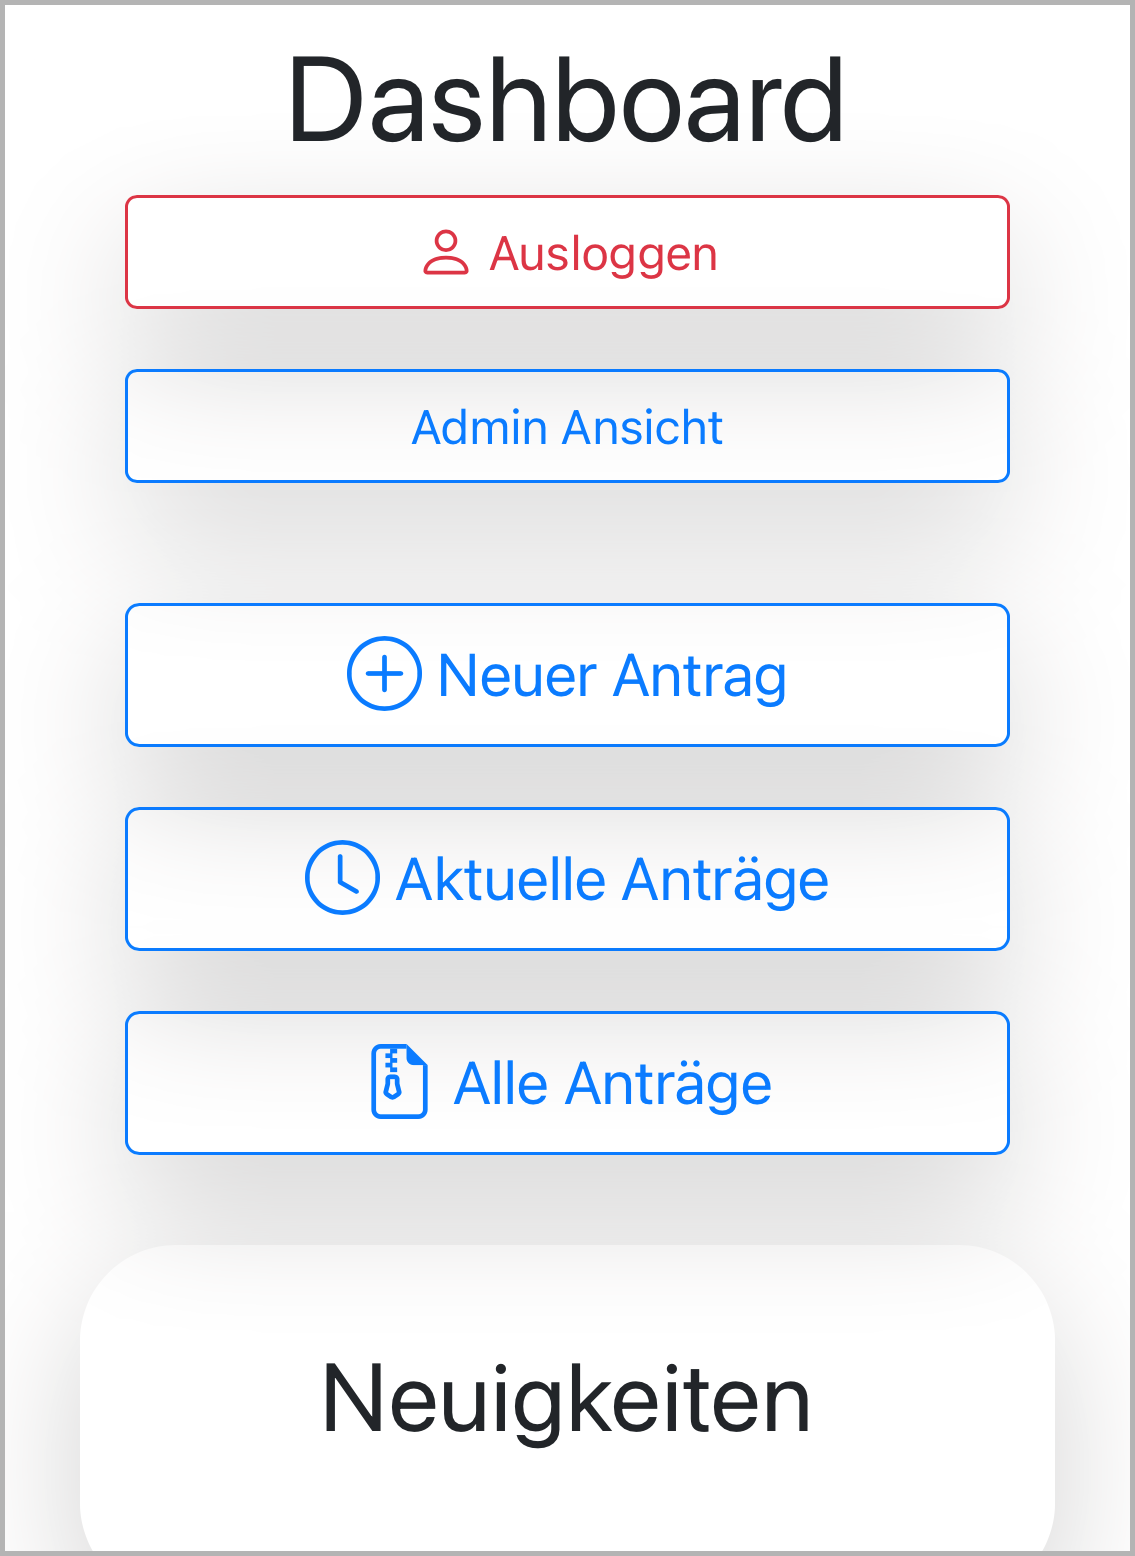
\includegraphics[width=0.4\linewidth]{images/website/dashboard_mobile}
	\caption[Dashboard Mobil]{Ein Bild der endgültigen Startseite (Mobil)}
	\label{fig:dashboardmobile}
\end{figure}

\paragraph{Menü-Element Desktop}
~\\
Der Container mit den Funktionselementen hat, wie beim Login, einen Schatten, der ihn von dem Hintergrund abhebt. In diesem Container befinden sich die Menübezeichnung und die klickbaren Elemente, die auch aus einem Container bestehen, sowie eine responsive Illustration, die zu der jeweiligen Funktion passt, welche mit einem Icon versehen ist. 
\begin{code}{html}
<b-col id="dash-main-cont" class="d-none d-md-block" cols="12" md="4">
	<b-container>
		<b-row
			id="dash-row"
			align-v="center"
			align-h="center"
			class="shadow-xl"
		>
			<b-col cols="12">
				<center><h2 id="menu-h2">Menü</h2></center>
			</b-col>
			<!-- Custom Button für einen neuen Antrag -->
			<b-col
				id="new"
				cols="12"
				class="shadow-lg dash-elem"
				v-on:click="newApplication"
			>
				<b-container style="height: 100%">
					<b-row align-h="center" align-v="center" style="height: 100%">
						<b-col cols="6" class="ill-wrapper d-none d-md-block">
						<!-- Illustration neuer Antrag -->
							<b-img
								id="all-ill"
								center
								src="@/assets/new.svg"
								alt="Illustration für alle Anträge"
							></b-img>
						</b-col>
						<b-col cols="12" md="6">
							<h2 id="new-h2" class="dh">Neuer Antrag</h2>
						</b-col>
					</b-row>
				</b-container>
			</b-col>
			
			...
		</b-row>
	</b-container>
</b-col>
\end{code}
\captionof{listing}{HTML-Code-Teile des Startseitenmenüs}
	\label{list:menuhtml} ~\\
Optisch wurde vor allem die Höhe des umschließenden Containers verändert und dessen umliegende Abstände. Wie man auf der \autoref{fig:dashboard} sehen kann, wurden auch die Ecken abgerundet. Nicht ersichtlich ist, dass sich die Funktionselemente optisch absenken und der Schatten entfernt und die Farbe verändert wird, wenn man mit der Maus, die sich zu einer zeigenden Hand verändert, über das Element fährt. 
\begin{code}{css}
#dash-main-cont {
	height: 70vh;
}

#dash-row {
	height: 70vh;
	padding-left: 2rem;
	padding-right: 2rem;
	padding-bottom: 1.5rem;
}

.dash-elem {
	background-color: rgb(255, 255, 255);
	height: 22%;
	transition: all 0.3s ease 0s;
	cursor: pointer;
	outline: none;
}

.dash-elem:hover {
	background-color: #8ff2ff;
	box-shadow: 0px 0px 50px rgba(0, 0, 0, 0.144);
	color: rgb(141, 141, 141);
	transform: translateY(3px);
}

#dash-row {
	border-radius: 6rem 6rem 6rem 6rem;
}
\end{code}
\captionof{listing}{Teile des CSS Codes, des Startseitenmenüs}
	\label{list:cssmenu} ~\\
\paragraph{Menü-Element Mobil}
~\\
Wie bereits erwähnt, ist die mobile Ansicht sehr schlicht gehalten, damit sie nicht überladen wirkt und sich auch vor allem die Lehrer, die sich nicht viel mit Technik beschäftigen auskennen. Daher wird auf der mobilen Ansicht nur das Nötigste angezeigt, siehe \autoref{fig:dashboardmobile} . Alle Knöpfe werden nun vertikal angeordnet und mit einem passenden Icon bestückt. Die Newselemente unterscheiden sich kaum von denen der Desktop-Version, die Elemente sind lediglich mit etwas weniger Details bestückt und nicht in einem scrollbaren Container, da man auf der mobilen Version sonst doppelt scrollen müsste.
\begin{code}{html}
	<!-- DASH MOBILE -->
	<b-col class="d-block d-md-none" cols="12">
	  <!-- Column -->
	  <b-container fluid>
		<b-row align-v="center" align-h="center">
		  <b-col cols="12">
			<center><h1 style="margin-top:10px;">Dashboard</h1></center>
		  </b-col>
		  <b-col cols="12">
			<!-- Logout Button -->
			<b-button
			  variant="outline-danger"
			  class="shadow-lg"
			  v-on:click="logout"
			  style="margin-top:0px; margin-bottom:20px; width:100%"
			>
			  <b-icon icon="person" aria-hidden="true"></b-icon> Ausloggen
			  <!-- Icon -->
			</b-button>
		  </b-col>
		  <b-col cols="12">
			<!-- Neuer Antrag Button --><b-button
			  size="lg"
			  variant="outline-primary"
			  v-on:click="newApplication"
			  class="shadow-lg"
			  style="margin-bottom:20px; width:100%"
			>
			  <b-icon icon="plus-circle" aria-hidden="true"></b-icon> Neuer
			  Antrag
			</b-button></b-col
		  >	
\end{code}
\captionof{listing}{Teile des HTML-Codes der mobilen Startseite}
	\label{list:startmobile} ~\\
\paragraph{Neuigkeiten-Element}
~\\
Die Neuigkeiten-Elemente sind mit einer Illustration bestückt, die den momentanen Status des jeweiligen Antrags beschreiben soll. Außerdem wird ein Titel der Neuigkeit mitgegeben, die zum Beispiel \enquote{Antrag X abgelehnt} heißen könnte. Etwas mehr Details werden noch in einem Beschreibungsfeld mitgegeben, das wegen der Übersichtlichkeit nur auf Desktopgeräten sichtbar ist.
\begin{code}{html}
	<b-row align-v="center">
	<b-col cols="2">
	  <b-container style="height: 100%">
		<b-row align-v="center" align-h="center" style="height: 100%">
		  <!-- Illustration Angenommen/Abgelehnt -->
		  <img
			src="@/assets/accepted_1.svg"
			class="align-middle news-status"
			style="height: 50px; width: auto"
			alt="Illustration von arbeitenden Personen"
		  />
		</b-row>
	  </b-container>
	</b-col>
	<b-col cols="10">
	  <b-container>
		<b-row align-h="center" align-v="center">
		  <b-col cols="12">
			<!-- Titel der Neuigkeit -->
			<h3 class="news-elem-heading">{{ snews.title }}</h3>
		  </b-col>
		</b-row>
		<b-row align-h="center" class="d-none d-md-block">
		  <b-col cols="12">
			<!-- Beschreibung der Neuigkeit -->
			<h4 class="news-elem-heading">{{ snews.description }}</h4>
		  </b-col>
		</b-row>
	  </b-container>
	</b-col>
  </b-row>	
\end{code}
\captionof{listing}{HTML Code, des Neuigkeiten Elementes}
	\label{list:htmlnews} ~\\
\newpage
\subsubsection{Neuer Antrag}
\label{chapter:implementierung-frontend-komponenten-neu}
Auf diese Seite gelangt der Nutzer entweder, durch die Betätigung des \textit{Neuer Antrag} Buttons auf der Startseite oder über die Verknüpfung auf der \textit{Alle Anträge} oder \textit{Aktive Anträge} Ansicht. Da es nicht möglich ist, ein einheitliches Formular zu kreieren, wurde vor dem Formular eine Auswahlmöglichkeit der Antragsart eingebaut.
\paragraph{Auswahl}
~\\
Die von uns gewählte Auswahlmöglichkeit ist sehr einfach und intuitiv gestaltet. Die drei verschiedenen Hauptarten von Anträgen sind klar und deutlich zu unterscheiden. Optisch sind die Knöpfe ähnlich strukturiert, wie die der Hauptseite. Damit zieht sich ein einheitliches Design durch die Website.
\begin{figure}[H]
	\centering
	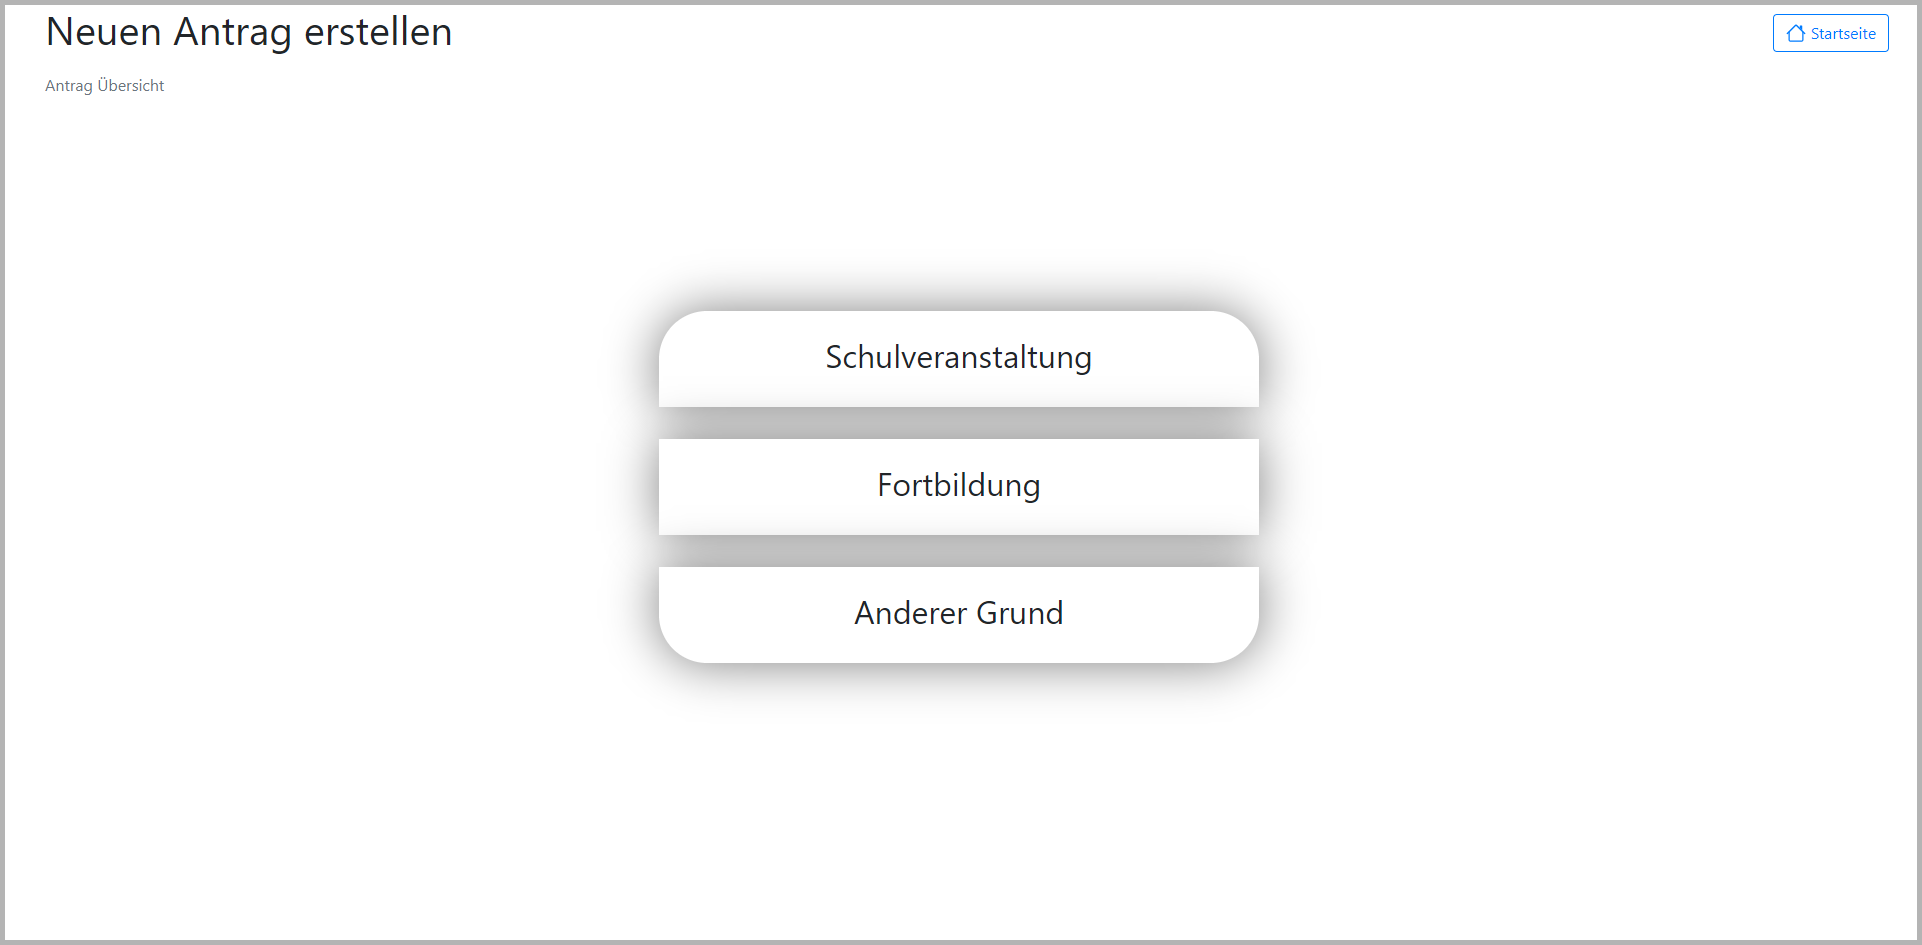
\includegraphics[width=1\linewidth]{images/website/neu}
	\caption[Neuer Antrag Auswahl]{Ein Bild der endgültigen Seite, um ein einen neuen Antrag auszuwählen}
	\label{fig:neuauswahl}
\end{figure}
Die Knöpfe sind in eigenen Containern dargestellt, um sie optimal der Größe des Endgerätes anzupassen. In dem Container, der sich mit einem Schatten vom Hintergrund abhebt, ist eine eindeutige Bezeichnung der Funktion, des jeweiligen Elementes. Fährt man mit der Maus über einen Knopf, wird dieser, wie auf der Startseite, in seiner Farbe verändert.
\begin{code}{html}
	<b-container id="school-button" class="na-elem shadow-xl">
	<!-- Custom Button zum erstellen eines Schulantrages -->
	<b-row
	  class="na-elem-sr"
	  align-v="center"
	  v-on:click="school()"
	>
	  <b-col cols="12">
		<h2 class="na-elem-h">Schulveranstaltung</h2>
	  </b-col>
	</b-row>
  </b-container>	
\end{code}
\captionof{listing}{HTML Code, einer Auswahlmöglichkeit}
	\label{list:htmlselect} ~\\
\paragraph{Schulveranstaltung}
~\\
Der Antrag für eine neue Schulveranstaltung ist der komplexeste Antrag mit den meisten Eingabefeldern. Außerdem gehören zu dem Antrag für eine Schulveranstaltung auch die Anträge der Begleitpersonen . Um die Eingabe von Uhrzeiten und Daten einfacher zu gestalten, wurden die Elemente \enquote{b-form-datepicker} und \enquote{b-form-timepicker} verwendet. Dies sind standardmäßige Elemente, die von BootstrapVue vordefiniert sind. Um eine korrekte Eingabe sicherzustellen, wurde alle Eingabefelder mit einem Titel und einer Zusatzinformation ausgestattet.
\begin{figure}[H]
	\centering
	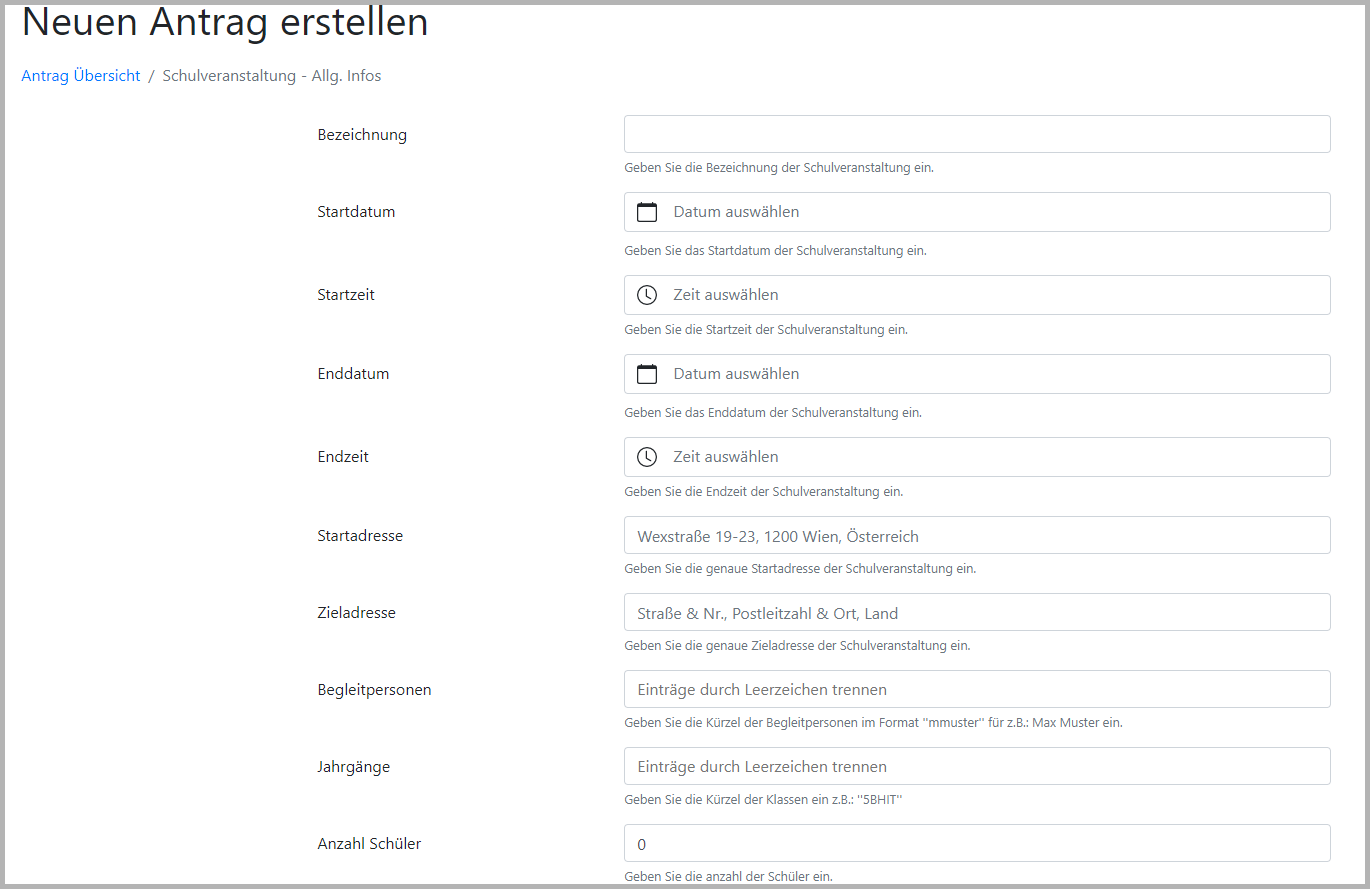
\includegraphics[width=1\linewidth]{images/website/schul_1}
	\caption[Neuer Schulantrag]{Ein Bild der Schulantrags Seite (Teil 1)}
	\label{fig:schulantrag1}
\end{figure}
\begin{figure}[H]
	\centering
	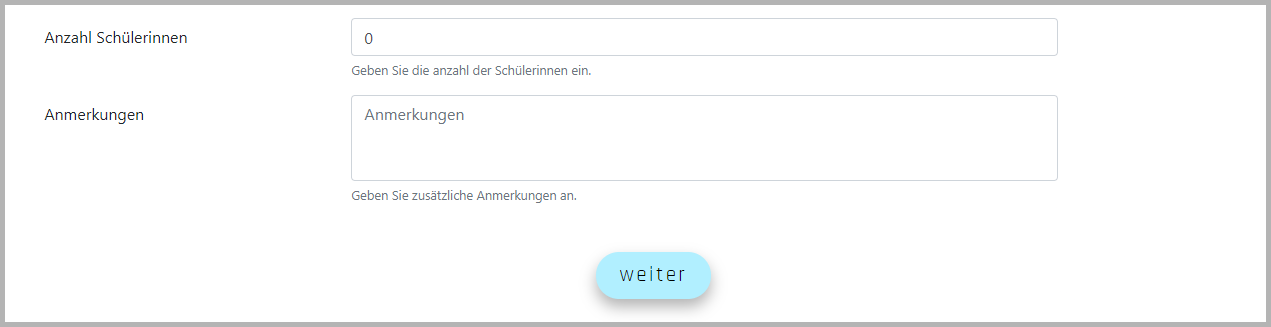
\includegraphics[width=1\linewidth]{images/website/schul_2}
	\caption[Neuer Schulantrag]{Ein Bild der Schulantrags Seite (Teil 2)}
	\label{fig:schulantrag2}
\end{figure}
Alle Eingabefelder sind in sogenannte \enquote{b-form-groups} eingefügt. Diese Elemente bieten die Möglichkeit, einen Titel, der in unserem Fall auf der linken Seite angebracht ist und eine Beschreibung, die unterhalb des Eingabefelds eingefügt ist, hinzugefügt. Diese Elemente sind ebenfalls responsiv. In der \enquote{form-group} wird das jeweilige Element eingefügt, welches man eigentlich einbauen will. Diese Elemente können unter anderem normale Eingabefelder sein, Checkboxe, Radiobuttons, Timepicker, Datepicker, etc.. 
\begin{code}{html}
	<b-form-group
        id="bez"
        label-cols-sm="4"
        label-cols-lg="3"
        content-cols-sm
        content-cols-lg="7"
        description="Geben Sie die Bezeichnung der Schulveranstaltung ein."
        label="Bezeichnung"
        label-for="bezeichnung"
    >
        <b-form-input
            id="bezeichnung"
            v-model="data.Name"
            :readonly="readonly"
            @input="updateData"
        ></b-form-input>
    </b-form-group>
\end{code}
\captionof{listing}{Beispiel für eine Eingabegruppe}
~\\
Das \textit{Timepicker} Element kann ganz einfach, wie im oberen Absatz beschrieben, in eine Eingabegruppe eingefügt werden. Da das Element von Bootstrap vordefiniert ist, muss man leidiglich die üblichen Werte, wie ID und Platzhalter, setzen. Das Einzige, was beachtet werden sollte, ist, dass man die richtige Zeitzone (Auflistung 7.13 locale) wählt.
\begin{code}{html}
	<b-form-timepicker
		id="stz"
		v-model="startTime"
		:readonly="readonly"
		@input="updateTime"
		locale="de"
		placeholder="Zeit auswählen"
  	></b-form-timepicker>
\end{code}
\captionof{listing}{Timepicker}
~\\
Der \textit{Datepicker} ist noch einfacher zu bedienen, als der \textit{Timepicker}. Hier sind nur die üblichen Parameter zu setzen.
\begin{code}{html}
	<b-form-datepicker
		id="end"
		v-model="endDate"
		:readonly="readonly"
		@input="updateTime"
		class="mb-2"
		placeholder="Datum auswählen"
  	></b-form-datepicker>
\end{code}
\captionof{listing}{Datepicker}
	\label{list:bspinputgroup} ~\\
Aus den, im Formular angegebenen Daten, wird automatisch ein weiteres Formular generiert. Dies geschieht, nachdem der \enquote{Weiter} Button betätigt wurde und alle Daten als valide anerkannt wurden. Das Formular beinhaltet für jede Begleitperson die geforderten Eingabefelder (\autoref{fig:schulantrag3}). Die Struktur dieser Elemente ist exakt die selbe, wie jene, der Elemente, die in \autoref{fig:schulantrag1} dargestellt wurden. 
\begin{figure}[H]
	\centering
	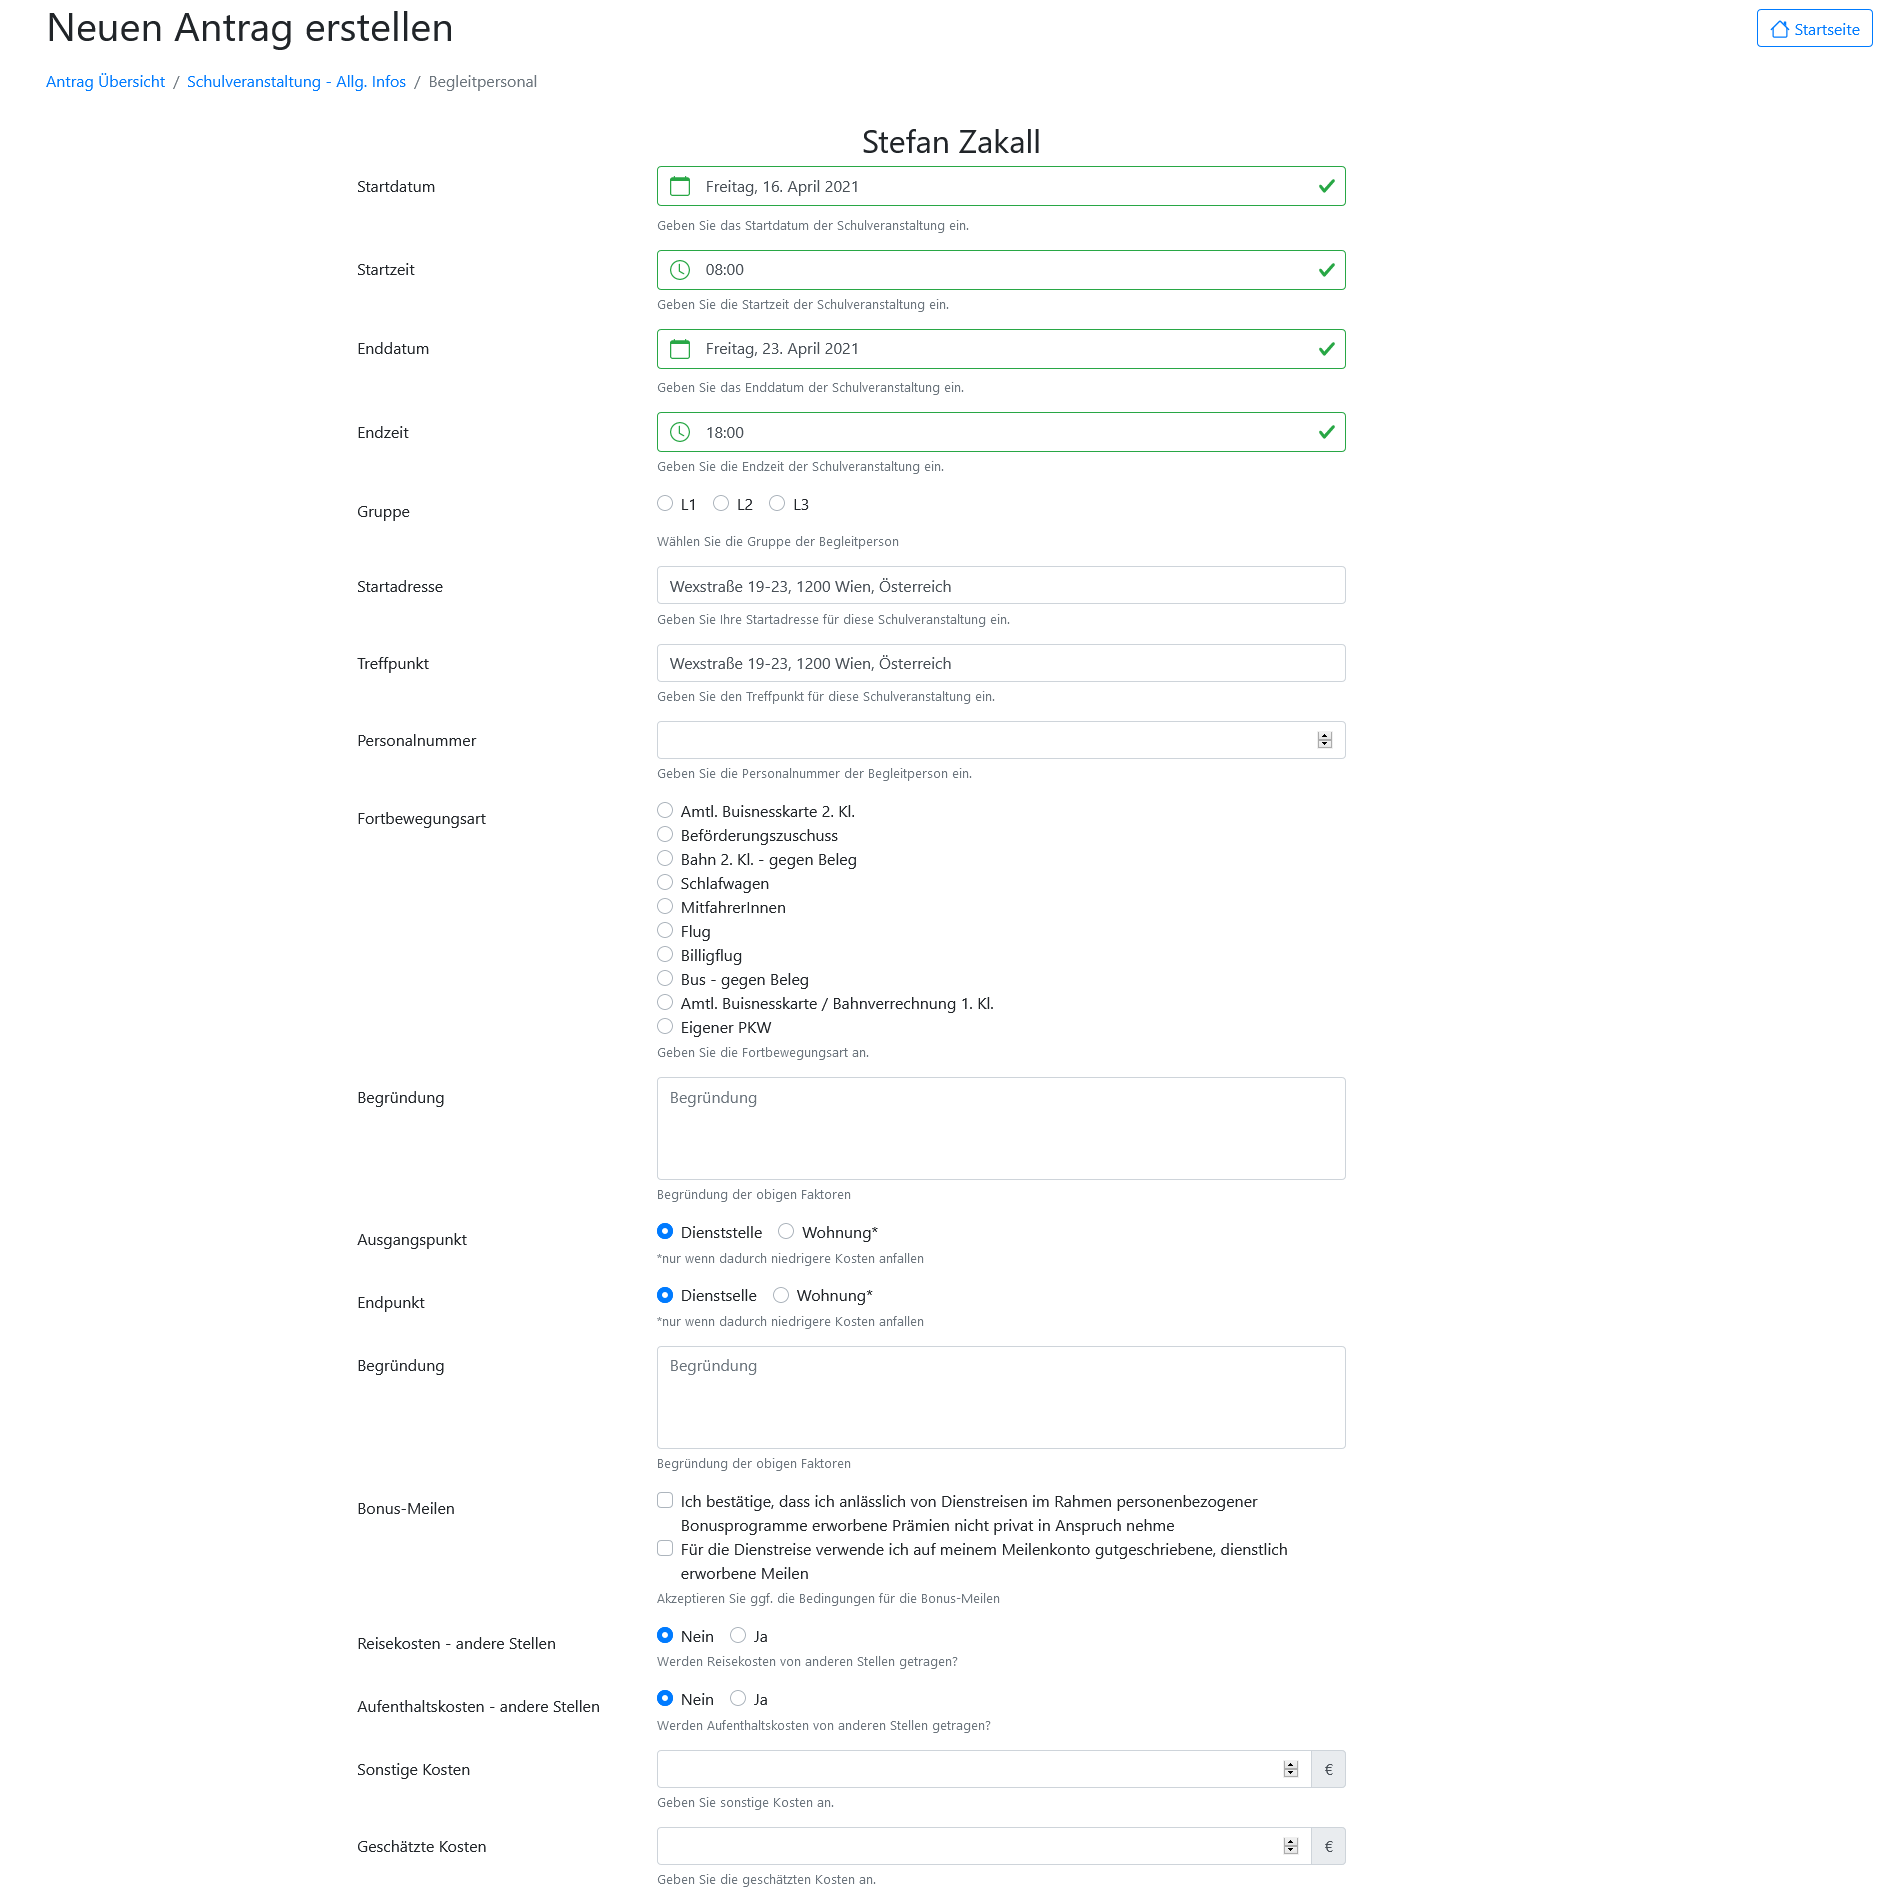
\includegraphics[width=1\linewidth]{images/website/schul_3_1}
	\caption[Neuer Schulantrag]{Ein Bild des Begleitformulars (Teil 1)}
	\label{fig:schulantrag3}
\end{figure}
\paragraph{Fortbildung}
~\\
Das Fortbildungsformular ist für Seminare, Tagungen, Lehrgänge und sonstige Events dieser Art gedacht. Um die Formulare einheitlich zu halten, wurde auch hier wieder die selbe Struktur der Eingabefelder verwendet. Falls man die sonstige Art auswählt, fügt sich automatisch eine zusätzliche Eingabe hinzu, in der man das Anliegen genauer spezifizieren kann.
\begin{figure}[H]
	\centering
	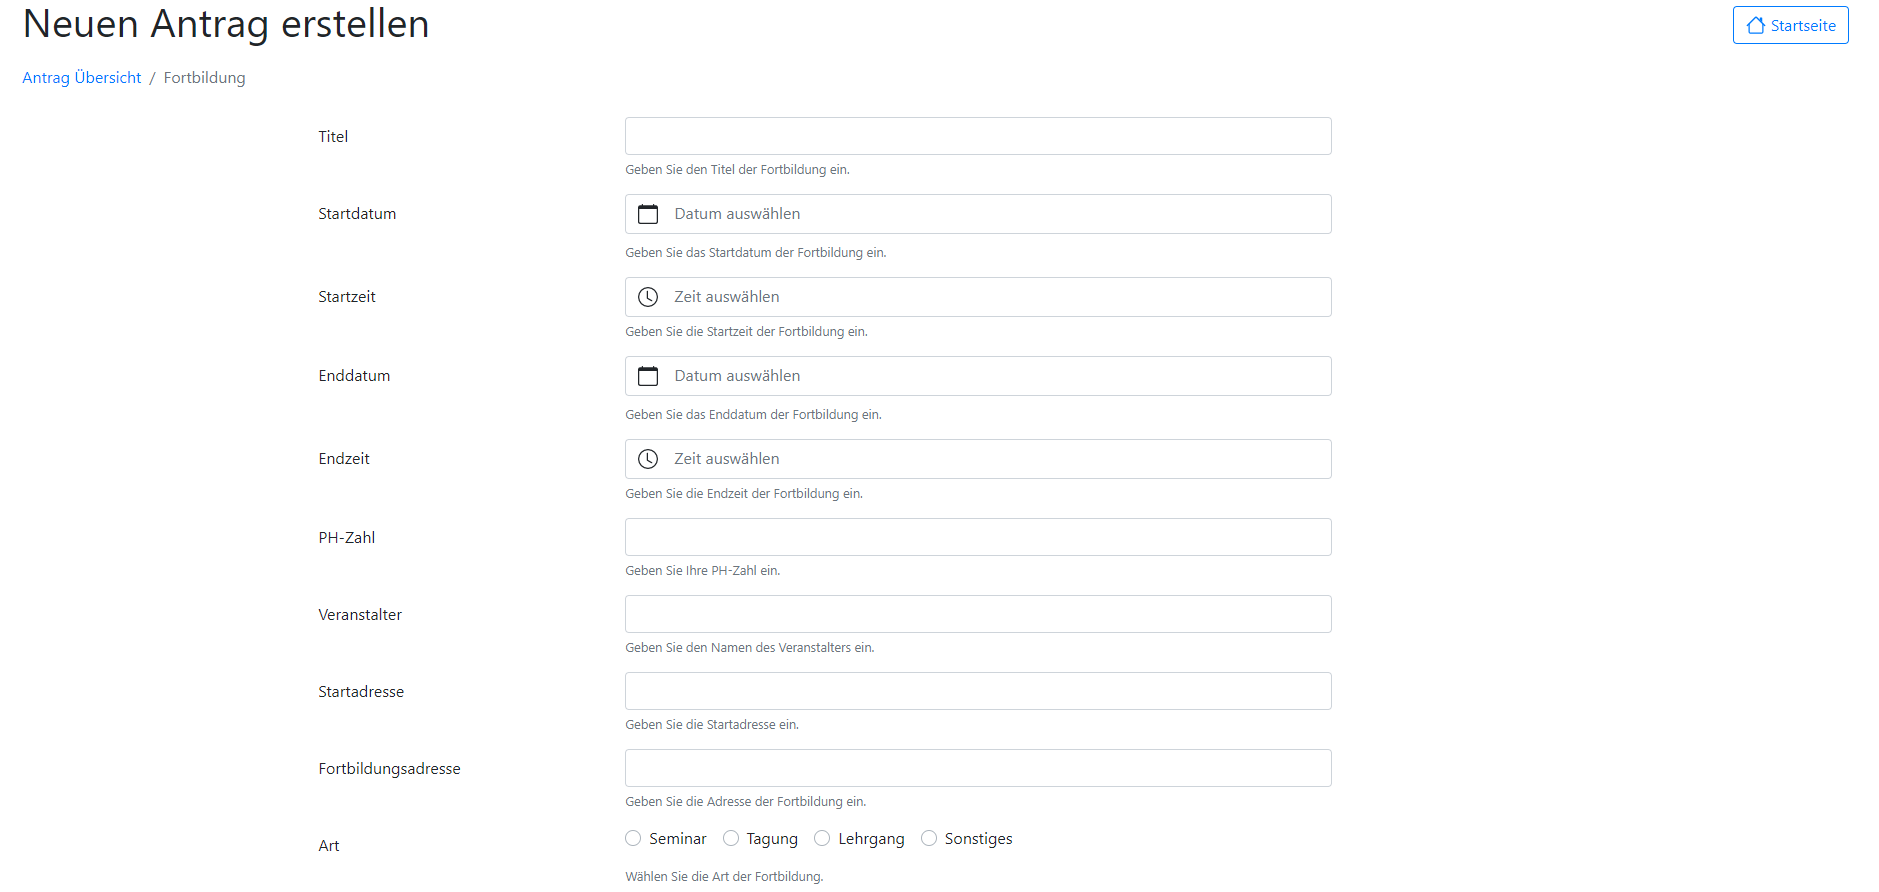
\includegraphics[width=1\linewidth]{images/website/fortbildung_1}
	\caption[Neuer Schulantrag]{Ein Bild des Begleitformulars (Teil 2)}
	\label{fig:frotbildung}
\end{figure}

\paragraph{Sonstige Anträge}
~\\
Zu den sonstigen Anträgen gehören Anliegen, wie Pflegefreistellungen, Dienstaufträge, Arzttermine und sonstige Freistellungen dieser Arten. Wählt man einen Dienstauftrag als Art aus, erscheinen automatisch noch Eingabefelder, die das Eingeben der GZ und des Titels, des Dienstauftrages ermöglichen.
\begin{figure}[H]
	\centering
	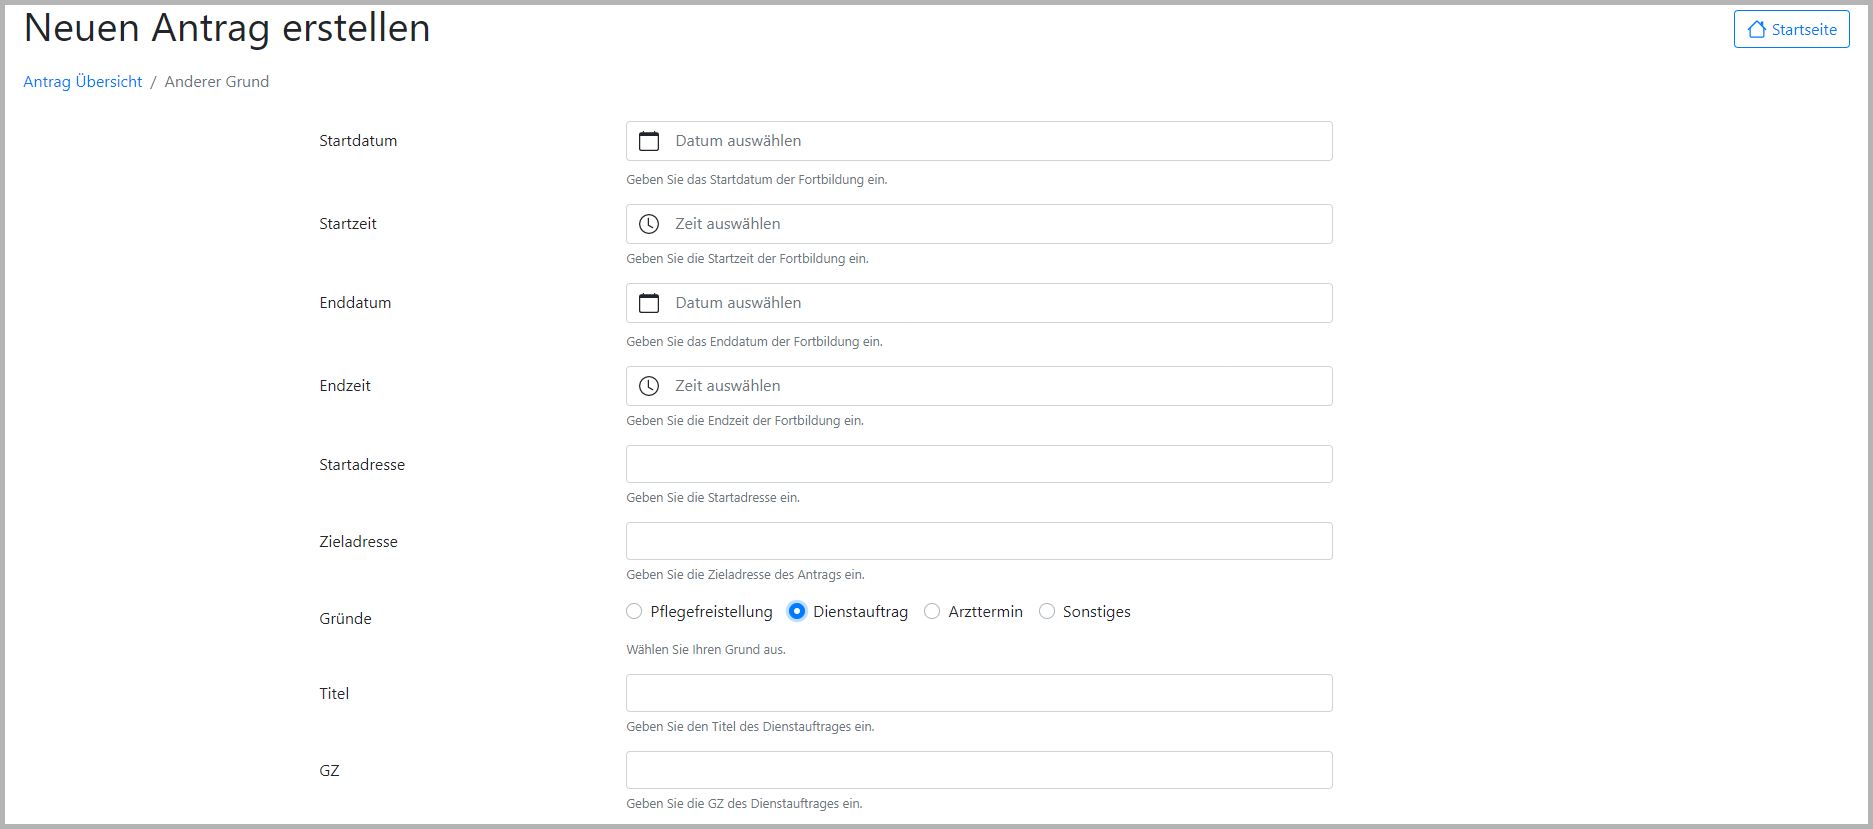
\includegraphics[width=1\linewidth]{images/website/dienstauftrag}
	\caption[Neuer Schulantrag]{Ein Bild des Begleitformulars (Teil 2)}
	\label{fig:dienst}
\end{figure}

\paragraph{Reiseantrag}
~\\
Der Reiseantrag wird automatisch bei den Formularen der Anträge angehangen, bei denen eine Reise nötig ist. Ist keine Reise für einen bestimmten Antrag (zum Beispiel ein Arztbesuch) vorgesehen, dann wird das Formular nicht angehangen und es müssen keine  Daten eingegeben werden. Die Struktur der Elemente ist ident zu denen, die bereits besprochen wurden.
\begin{figure}[H]
	\centering
	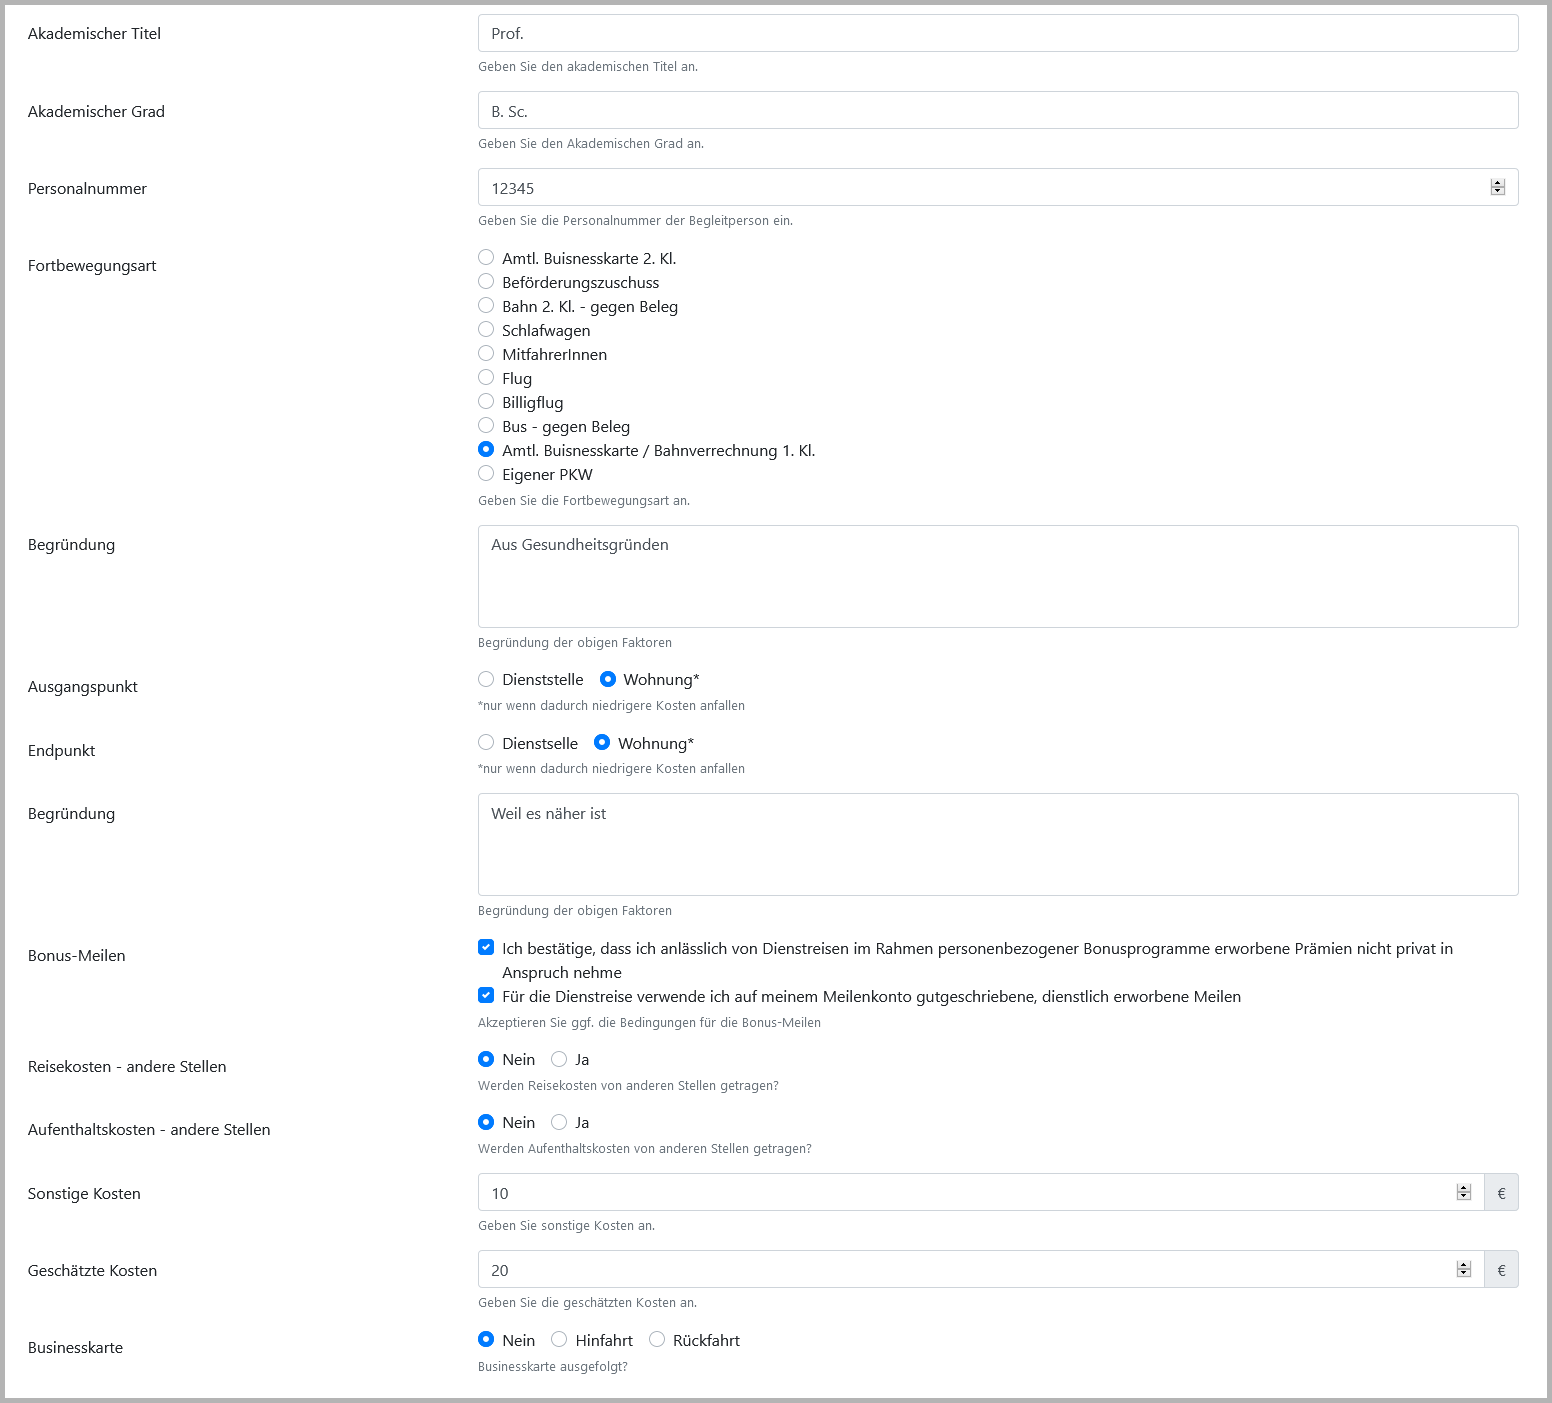
\includegraphics[width=1\linewidth]{images/website/zusatz_1}
	\caption[Neuer Schulantrag]{Ein Bild des Reiseantrages (Teil 2)}
	\label{fig:zusatz1}
\end{figure}

\subsubsection{Reisekostenabrechnung}
\label{chapter:implementierung-frontend-komponenten-rechnung}
Das Formular der Reisekostenabrechnung fordert sehr viele verschiedene Werte von den Lehrern. Durch die Unterstützung der Website, ist das Eingeben der Daten wesentlich einfacher, als auf dem Papier, da gewisse Felder, je nach Eingabe des Benutzers, automatisch ausgegraut werden. Wenn zum Beispiel die Tabelle in \autoref{fig:reiserechnungsite} betrachtet wird, kann man nur in jene Felder schreiben, die man mit den Checkboxen angeklickt hat. Außerdem können direkt digital Belege an die Reisekostenabrechnung anhängt werden. Zudem wird automatisch die Zeitspanne des jeweiligen Antrages berechnet und entsprechend viele Zeilen in der Tabelle erzeugt.
\begin{figure}[H]
	\centering
	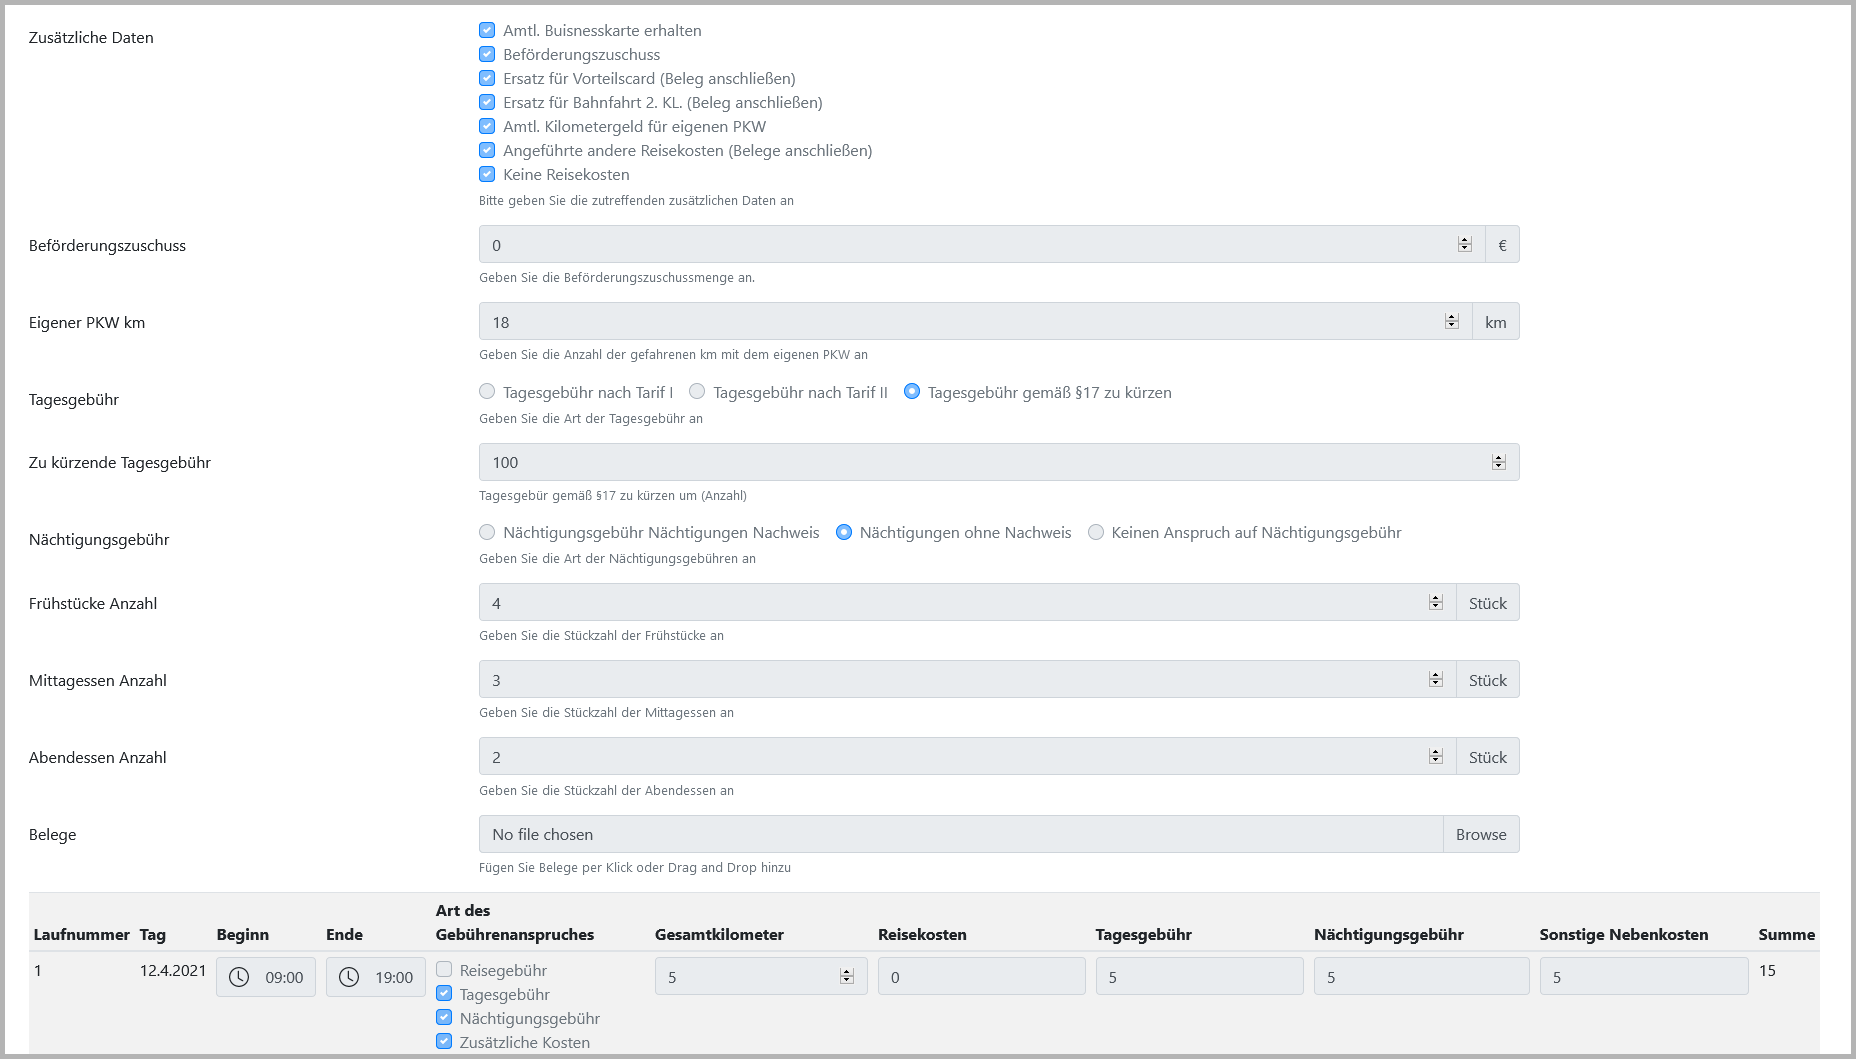
\includegraphics[width=1\linewidth]{images/website/reiserechnung_1}
	\caption[Neuer Schulantrag]{Ein Bild der Reiserechnung}
	\label{fig:reiserechnungsite}
\end{figure}
In \autoref{fig:reiserechnungsite} wurden Elemente verwendet, die uns im Gegensatz zu normalen Eingaben nicht bekannt sind, einerseits Tabellen, andererseits die Dateiauswahl.
\paragraph{Dateiauswahl}
~\\
Wie auch bei den anderen Elementen der Formulare, wie zum Beispiel bei dem \textit{Timepicker}, hat Bootstrap ein veorgefertigtes Element für die Dateiauswahl. 
\begin{code}{html}
	<!-- Belege Input -->
	<b-form-group
	  id="belg"
	  label-cols-sm="4"
	  label-cols-lg="3"
	  content-cols-sm
	  content-cols-lg="7"
	  description="Fügen Sie Belege per Klick oder Drag and Drop hinzu"
	  label="Belege"
	  label-for="bel"
	>
	  <b-form-file
		multiple
		id="bel"
		v-model="invoices"
		v-on:input="convert"
		:disabled="readonly"
	  >
		<template slot="file-name" slot-scope="{ names }">
		  <b-badge variant="dark">{{ names[0] }}</b-badge>
		  <b-badge v-if="names.length > 1" variant="dark" class="ml-1">
			+ {{ names.length - 1 }} More files
		  </b-badge>
		</template>
	  </b-form-file>
	</b-form-group>
\end{code}
\captionof{listing}{Code - Datei auswählen}
	\label{list:dateiselect} ~\\
Wie auch andere Elemente, wird das Element zum Hochladen von Dateien in eine Eingabegruppe, mit Titel und Beschreibung eingesetzt. Nach dem Einsetzen des Elementes, kann sofort per Klick oder Drag and Drop eine, oder mehrere Dateien hinzugefügt werden.
\paragraph{Tabelle}
~\\
Um eine Tabelle zu erstellen, kann das Element \enquote{b-table} von Bootstrap benutzt werden. In diesem kann man direkt definieren, wie groß die Tabelle sein soll, was auf mobilen Geräten passieren soll, ob die Tabelle gestreift ist, oder nicht und noch weitere Parameter. In diesem Element, wurden die verschiedenen Spalten eingebaut. Dies wurde wie folgt umgesetzt:
\begin{code}{html}
	<b-table
          striped
          :items="data.items"
          :fields="fields"
          stacked="md"
          show-empty
          small
    >

		...

		<template #cell(start)="data">
			<b-form-timepicker
				style="min-width: 100px;"
				id="begin"
				locale="de"
				placeholder="Zeit"
				v-model="data.item.start"
				:readonly="readonly"
				v-on:input="update()"
			></b-form-timepicker>
		</template>

		...

	</b-table>
\end{code}
\captionof{listing}{Beispielcode Tabelle}
	\label{list:bsptable} ~\\
Die Spalten werden mittels \textit{Templates} erzeugt. Danach können variabel Werte in jene Spalte, bzw. in jeder Zeile eingefügt werden. In diesem Fall befindet sich in der Zelle ein \textit{Timepicker}, welcher zum Auswählen der Startzeit dient.
\newpage
\subsubsection{Ansicht aktive Anträge}
\label{chapter:implementierung-frontend-komponenten-aktiv}
Um den Lehrern das Betrachten von aktiven Anträgen einfacher zu machen, wurde eine extra Seite erstellt, die über das Menü auf der Startseite erreichbar ist. Hier werden alle aktiven Anträge (ein Antrag gilt als \enquote{aktiv}, von der Antragsstellung, bis zur Rechnungsphase). Der Benutzer sieht mittels Farben auf den ersten Blick, welchen Status der jeweilige Antrag hat, Rot: Antrag wurde abgelehnt, Gelb: Antrag wird bearbeitet, Grün: Antrag wurde angenommen. Außerdem werden in der Tabelle, der Titel des Antrages, der Leiter, das Einreichdatum und der genaue Status (In Bearbeitung, Rechnungsphase, ...) angezeigt. Falls der Benutzer viele Anträge auf einmal hat, wurde eine Funktion zum Suchen von Anträgen im oberen Teil der Seite eingebaut. Ebenfalls ist es möglich, jede Spalte auf- und absteigend zu sortieren. Falls der Knopf namens \enquote{Antrag betrachten} betätigt wurde, kommt der Nutzer auf die \enquote{Antrags Ansicht}.
\begin{figure}[H]
	\centering
	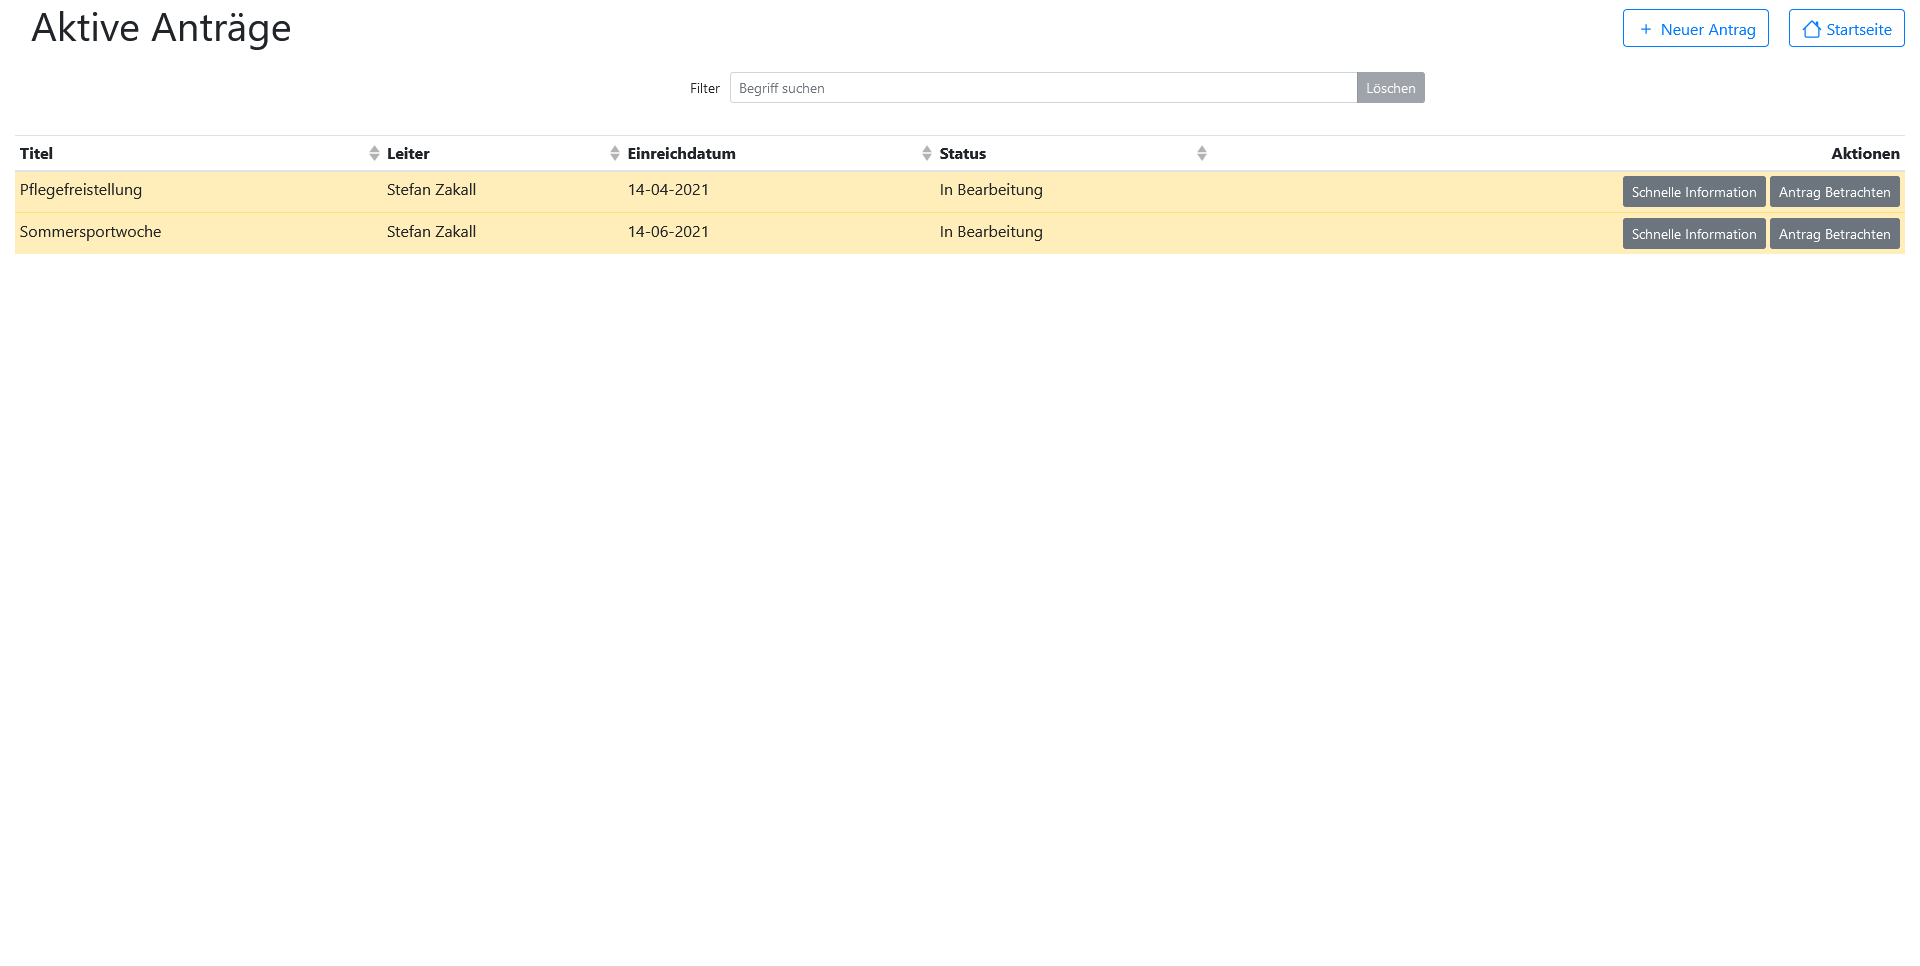
\includegraphics[width=1\linewidth]{images/website/aktiv}
	\caption[Aktiv]{Ein Bild der aktiven Anträge Seite}
	\label{fig:antragaktiv}
\end{figure}
Um die oben genannten Daten in einer geordneten Liste zu sehen, kann der Lehrer auf \enquote{Schnelle Information} klicken. Dieser Vorgang öffnet folgendes Fenster:
\begin{figure}[H]
	\centering
	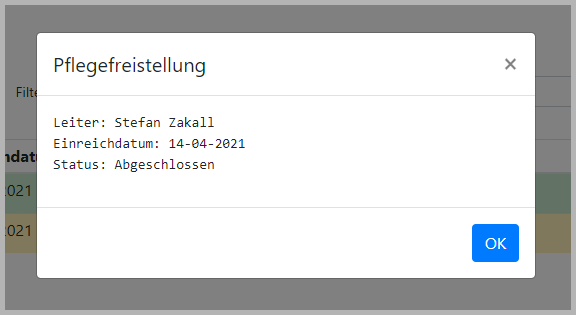
\includegraphics[width=0.6\linewidth]{images/website/aktiv_detail}
	\caption[Aktiv]{Ein Bild der Detail-Ansicht der aktiven Anträge Seite}
	\label{fig:antragaktivdetail}
\end{figure}
\paragraph{Such-Funktion}
~\\
Die Erstellung der Suchfunktion wurde wieder essentiell von den BootstrapVue Komponenten unterstützt. Es mussten eine Eingabegruppe erstellt werden, die ein Eingabefeld mit dem Typ \textit{\enquote{search}} hat. Um eine Eingabe schneller zu löschen wurde noch ein Knopf hinzugefügt, der erscheint, sobald man etwas eintippt. Durch die gute Integration von Bootstrap in VueJS war die Implementierung der Suchfunktion für die Tabelle reibungslos. Die Vergabe der Funktionalität der Such-Funktion wurde im Backend/Frontend Teil umgesetzt.
\begin{code}{html}
	<!-- Such Element -->
    <b-row align-h="center" style="margin-top: 1rem; margin-bottom: 2rem">
      <b-col cols="12" md="6">
        <b-form-group
          label="Filter"
          label-for="filter-input"
          label-cols-sm="3"
          label-align-sm="right"
          label-size="sm"
          class="mb-0"
        >
          <b-input-group size="sm">
            <b-form-input
              id="filter-input"
              v-model="filter"
              type="search"
              placeholder="Begriff suchen"
            ></b-form-input>

            <b-input-group-append>
              <b-button :disabled="!filter" @click="filter = ''"
                >Löschen</b-button
              >
            </b-input-group-append>
          </b-input-group>
        </b-form-group>
      </b-col>
    </b-row>
\end{code}
\captionof{listing}{Code - Anträge Suchfunktion}
	\label{list:antragsearchcode} ~\\
\paragraph{Filterbare Tabelle}
~\\
Die Aktivierung der filterbaren Tabelle ist mittels \textit{BootstrapVue} möglich. Dazu wurden folgende drei Festlegungen im \textit{\enquote{b-table}} Element hinzufügen:
\begin{code}{html}
	<b-table
		...
		:sort-by.sync="sortBy"
      	:sort-desc.sync="sortDesc"
      	:sort-direction="sortDirection"
		...
	>
	...
	</b-table>
\end{code}
\captionof{listing}{Code - Anträge filtern}
	\label{list:antragfiltercode} ~\\
\paragraph{Pop-Up Fenster}
~\\
Das Pop-Up Fenster wurde mittels einem \enquote{Modal} von Bootstrap verwirklicht. Dieses kann über einen zugewiesenen Button geöffnet werden und beinhaltet, je nach Antrag, dessen spezifische Daten.
\begin{code}{html}
	<!-- Info modal -->
    <b-modal
      :id="infoModal.id"
      :title="infoModal.title"
      ok-only
      @hide="resetInfoModal"
    >
      <pre>{{ infoModal.content }}</pre>
    </b-modal>
\end{code}
\captionof{listing}{Code - Pop-Up Fenster}
	\label{list:codepopup} ~\\

\subsubsection{Ansicht Alle Anträge}
\label{chapter:implementierung-frontend-komponenten-alle}
Diese Seite ist sehr ähnlich zu der \enquote{Aktive Anträge} Seite. Der Unterschied ist, dass der Nutzer hier auch bereits abgeschlossene Anträge sieht. Auch hier wurde die \enquote{Suchen} Funktion eingebaut, die hier eine wesentlich wichtigere Rolle spielt, als bei der Seite, der aktiven Anträge. Auch das Filtern der einzelnen Spalten ist wieder möglich.
\begin{figure}[H]
	\centering
	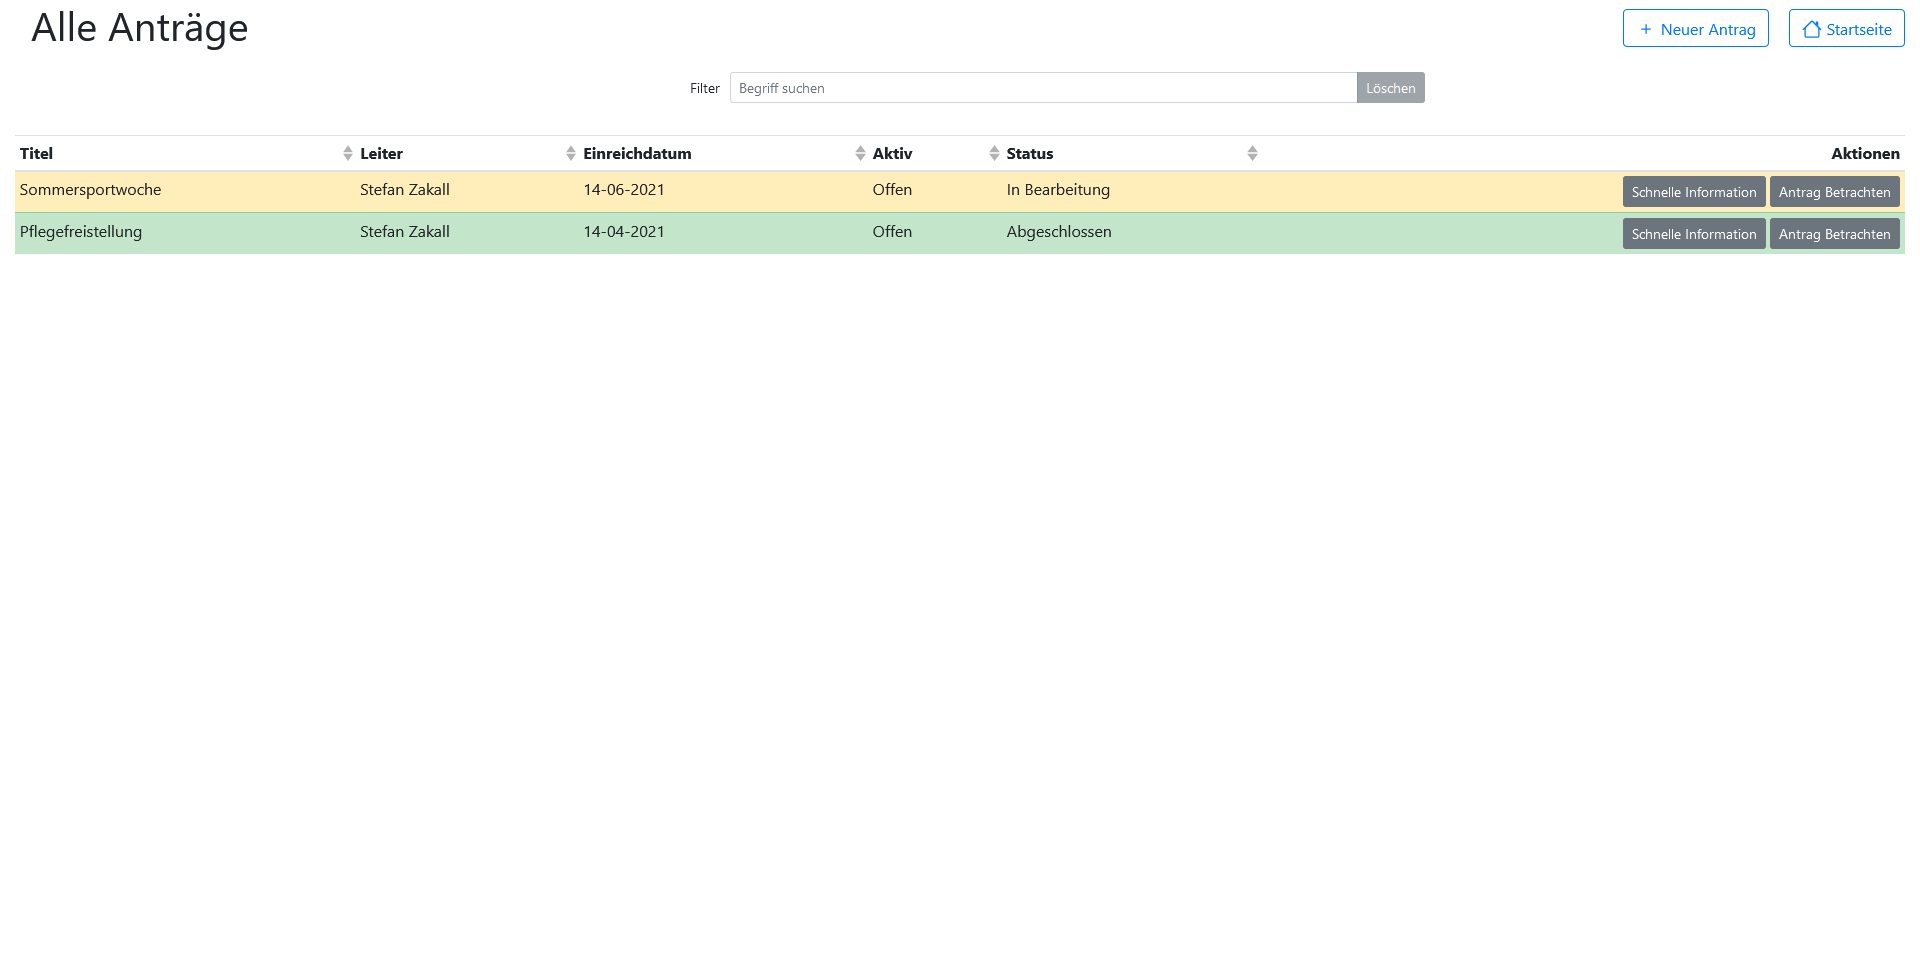
\includegraphics[width=1\linewidth]{images/website/alle}
	\caption[Aktiv]{Ein Bild der alle Anträge Seite}
	\label{fig:antragalle}
\end{figure}
~\\

\newpage
\subsubsection{Antragsansicht}
\label{chapter:implementierung-frontend-komponenten-antragsansicht}
Die Antragsansicht bietet den Nutzern alle möglichen Informationen zu ihrem Antrag, die sie brauchen. Um den Nutzern einen besseren Überblick zu schaffen, in welcher Phase sich ihr Antrag befindet, wurde eine Fortschrittsanzeige als erstes Element auf der Seite eingebaut. Desweiteren findet der Benutzer eine aufklappbare Liste auf der Seite, in der je nach Status des Antrages, die Daten angezeigt und/oder editiert werden können. Außerdem bietet diese Seite die Funktion, eine generierte PDF-Datei von jedem Antrag zu öffnen. Falls der Nutzer Daten geändert hat, kann er diese Änderung mit einem Knopf, der sich am Schluss der Website befindet speichern. Ebenfalls ist es möglich den Antrag zu schließen, hierbei öffnet sich aber eine Warnmeldung, in der man das Schließen des Antrages nochmal bestätigen muss.
\begin{figure}[H]
	\centering
	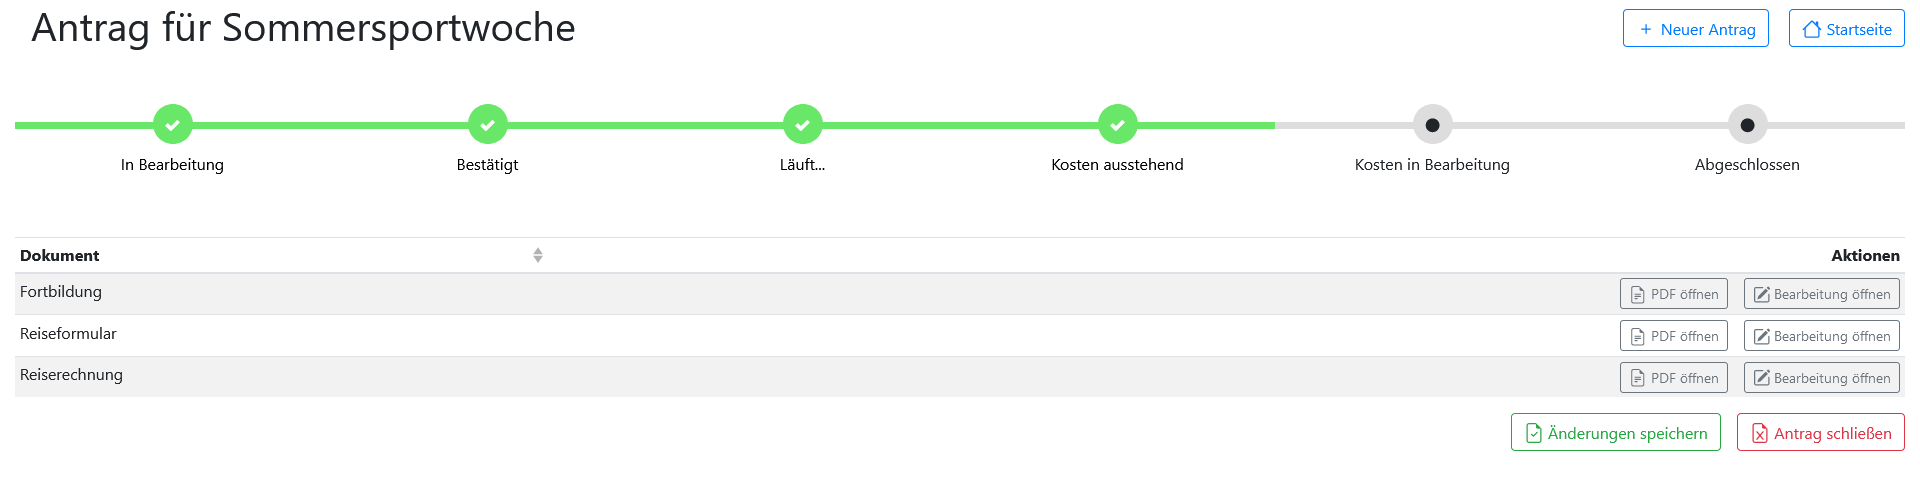
\includegraphics[width=1\linewidth]{images/website/antrag_zu}
	\caption[Aktiv]{Ein Bild der Detail-Ansicht der aktiven Anträge Seite}
	\label{fig:antragaktivdetail}
\end{figure}
\begin{figure}[H]
	\centering
	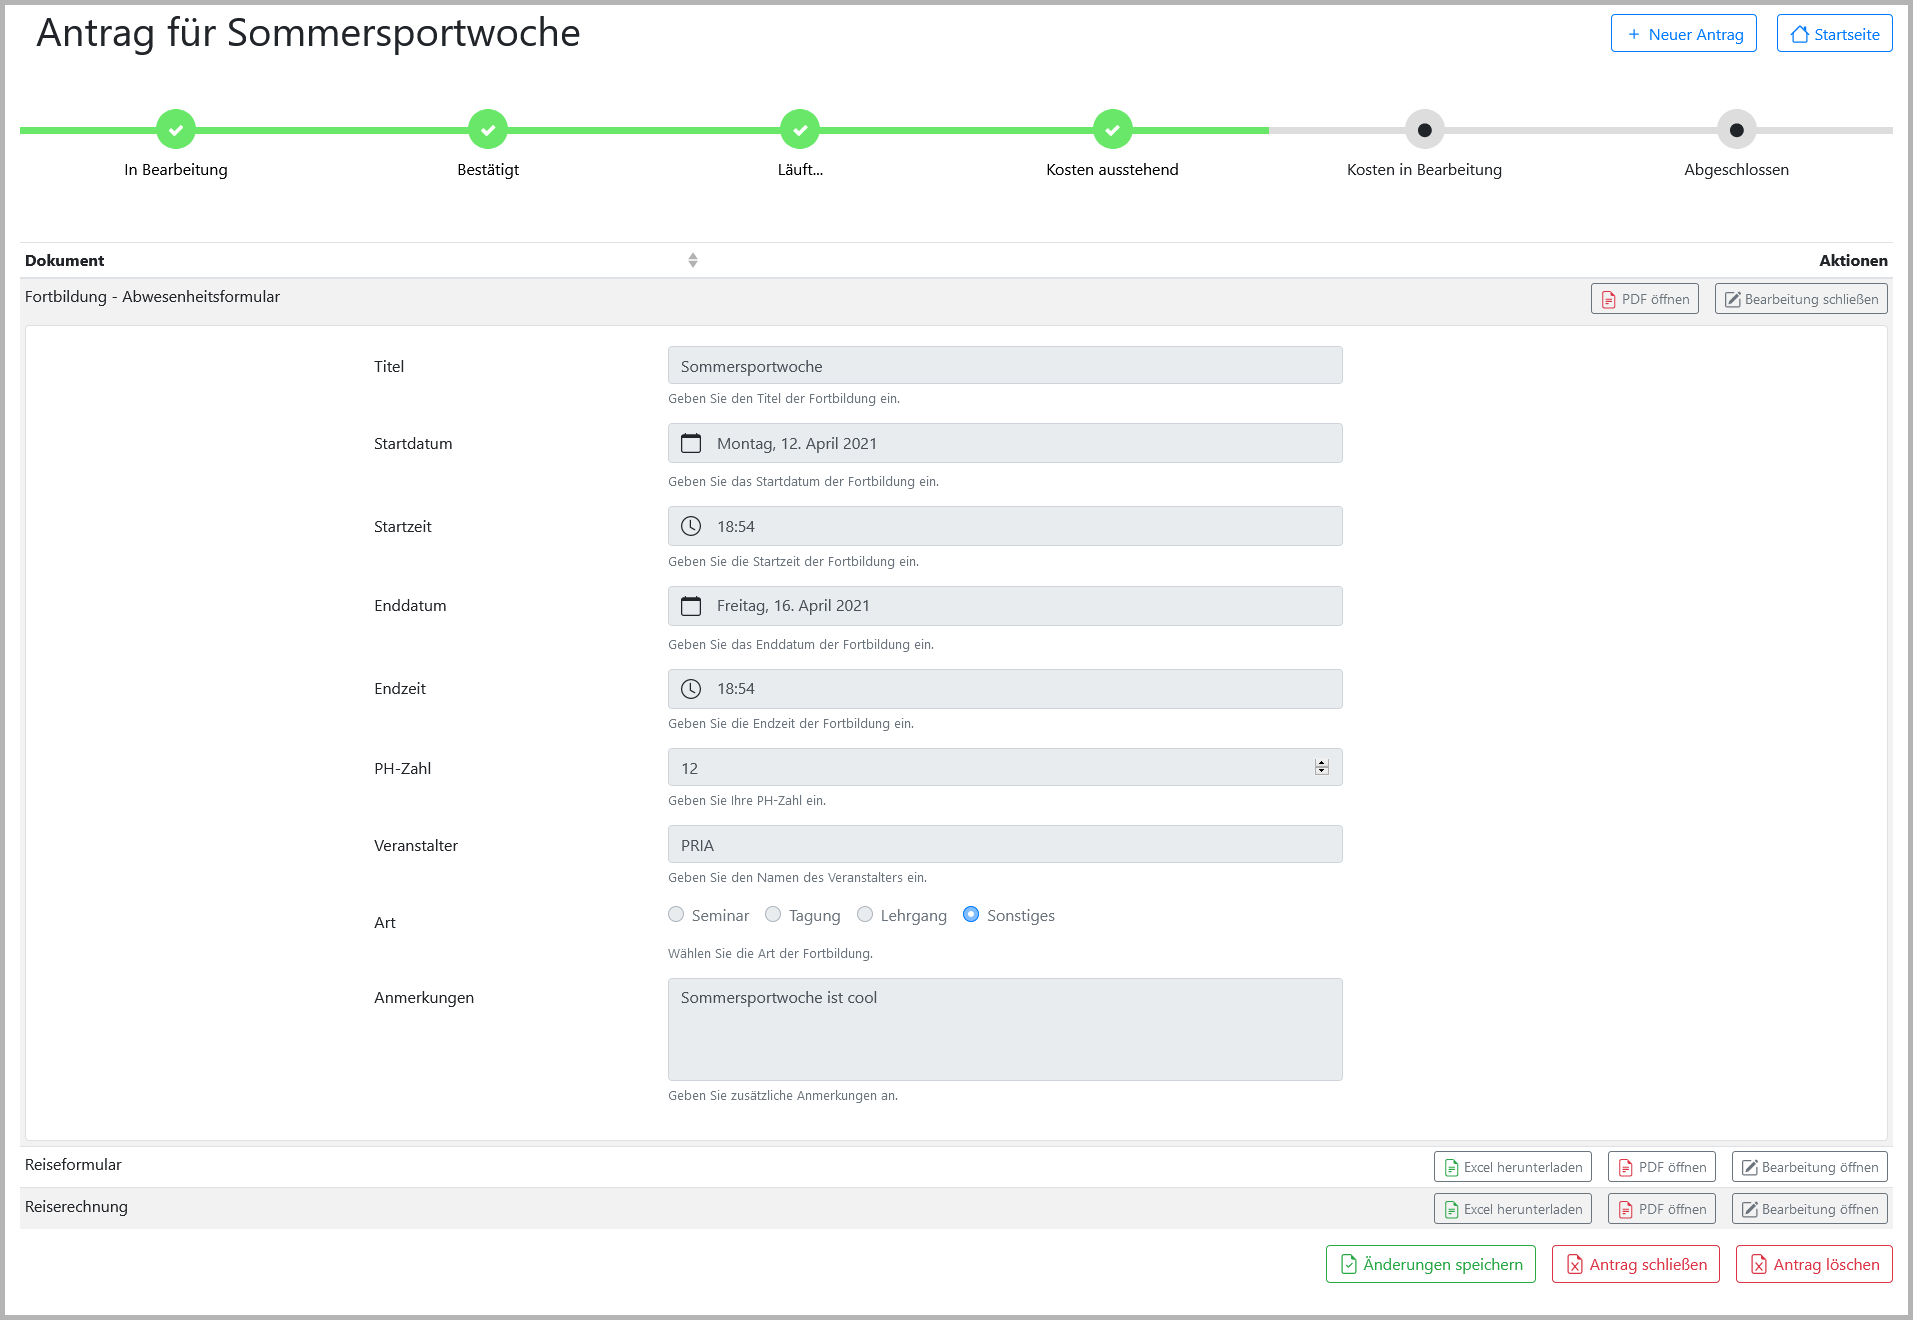
\includegraphics[width=1\linewidth]{images/website/antrag}
	\caption[Aktiv]{Ein Bild der Detail-Ansicht der aktiven Anträge Seite}
	\label{fig:antragaktivdetail}
\end{figure}
\begin{figure}[H]
	\centering
	
\includegraphics[width=0.6\linewidth]{images/website/antrag_schliessen}
	\caption[Aktiv]{Ein Bild der Detail-Ansicht der aktiven Anträge Seite}
	\label{fig:antragaktivdetail}
\end{figure}

~\\
\paragraph{Fortschrittsanzeige}
~\\
Ein Schritt der Fortschrittsanzeige besteht aus einem \enquote{div}, in dem sich ein \enquote{span} befindet. Das \enquote{div} ist ein \enquote{Strich} und in dem \enquote{span} befindet sich ein Icon, welches den Zustand beschreibt. Je nach Status des Fortschritts wird die Farbe mittels CSS-Klassen geändert.
\begin{code}{html}
	<div
            :class="{
              active: progress >= 1
            }"
            class="step"
          >
            <span class="icon">
              <i
                :class="{
                  'fa-check': progress >= 1,
                  'fa-circle': progress < 1 && progress > 0,
                  'fa-exclamation': progress == 0
                }"
                class="fa"
              ></i>
            </span>
            <span class="text text-truncate d-none d-md-block"
              >Einreichung</span
            >
          </div>
\end{code}
\captionof{listing}{Codeausschnitt - Fortschrittsanzeige}
	\label{list:codeprogress} ~\\

\begin{code}{css}
.track .step.fail:before {
  background: #ff3e3e;
}

.track .step.fail .icon {
  background: #ff3e3e;
  color: #fff;
}

.track .step.active .icon {
  background: #69e769;
  color: #fff;
}

.track .step.active:before {
  background: #69e769;
}
\end{code}
\captionof{listing}{CSS - Fortschrittsanzeige Farbklassen}
	\label{list:progresscolor} ~\\

\paragraph{Dokumente anzeigen}
~\\
Die verschiedenen Dokumente, die zu einem gewissen Antrag angehören, werden in einer Tabelle gelistet. Falls der Nutzer auf den \enquote{Bearbeitung öffnen} Knopf drückt, wird der Tabelle eine weitere Reihe hinzugefügt, die alle Informationen zu dem jeweiligen Antrag beinhaltet. Mittels VueJS wurden die bestehenden Formulare (hier als Beispiel einen Schulveranstaltungsantrag), in der Tabelle eingebunden und die Eingabefelder über die Datenschnittstelle (\autoref{chapter:implementierung-datenschnittstelle}) mit Daten befüllt.
\begin{code}{html}
	<template #row-details="row">
        <b-card>
            <!-- Schulveranstaltung -->
            <SchoolGeneral
            v-bind:readonly="sgreadonly"
            v-bind:data="app"
            v-bind:token="token"
            v-bind:url="url"
            v-on:update="updateSG"
            v-if="isLeader && row.item.title == 'Allgemeine Infos'"
            />
		</b-card>
	</template>
\end{code}
\captionof{listing}{Code - Dokumente anzeigen}
	\label{list:docanz} ~\\

\paragraph{Funktionen}
~\\
Wird der \enquote{Antrag schließen} Knopf betätigt, erscheint eine Sicherheitsmeldung. Diese wird mit einem \enquote{Modal} erstellt, welches einen Text beinhaltet, der den Nutzer vor den Folgen seiner Tat informiert und zwei weitere Knöpfe: ein grüner Knopf, um den Vorgang abzubrechen und einen roten Knopf, der einen rot blinkenden \enquote{Spinner} beinhaltet.
\begin{code}{html}
	<!-- Sicherheitshinweis Antrag schließen -->
    <b-modal ref="close-modal" hide-footer title="Antrag schließen">
      <b-container fluid>
        <b-row
          ><b-col cols="12">
            <div class="d-block text-center">
              <p>
                Sind Sie sich sicher, dass Sie den Antrag schließen wollen? Er
                wird danach nicht mehr für die Prüfer sichtbar sein und
                <b>kann nicht mehr geöffnet werden!</b>
              </p>
            </div>
          </b-col></b-row
        >
        <b-row>
          <b-col cols="6">
            <!-- Antrag schließen bestätigung -->
            <b-button class="mt-2" variant="outline-danger" block @click="delAn"
              >Antrag schließen <b-spinner small type="grow"></b-spinner
            ></b-button>
          </b-col>
          <b-col cols="6">
            <!-- Abbrechen Button --><b-button
              class="mt-2"
              variant="outline-success"
              block
              @click="hideClose"
              >Abbrechen</b-button
            ></b-col
          >
        </b-row>
      </b-container>
    </b-modal>
\end{code}
\captionof{listing}{Code - Antrag schließen Sicherheitshinweis}
	\label{list:securityalert} ~\\
~\\

\newpage
\subsubsection{Administrator Ansicht}
\label{chapter:implementierung-frontend-komponenten-admin}
Die Administratoransicht ist, wie die \enquote{alle Anträge} oder \enquote{aktive Anträge} Ansicht der Nutzer mit der Struktur einer Tabelle aufgebaut und verfügt über eine Such- als auch Filterfunktion. Eine Zusatzfunktion, damit man direkt in der Übersicht, einen oder mehrere Anträge auswählen kann und diese direkt als PDFs exportieren kann. Außerdem sehen die Admitistratoren auf den ersten Blick wesentlich mehr Informationen, als normale Nutzer. Es wird der Titel des Antrages angezeigt, die Art, das Enreichdatum, für wann der Antrag ist, den Status (je nach Status sehen gewisse Rollen die Anträge) und den Antragssteller in Kurzschreibweise. Auch hier ist es wieder möglich die Antragsansicht zu öffnen.
\begin{figure}[H]
	\centering
	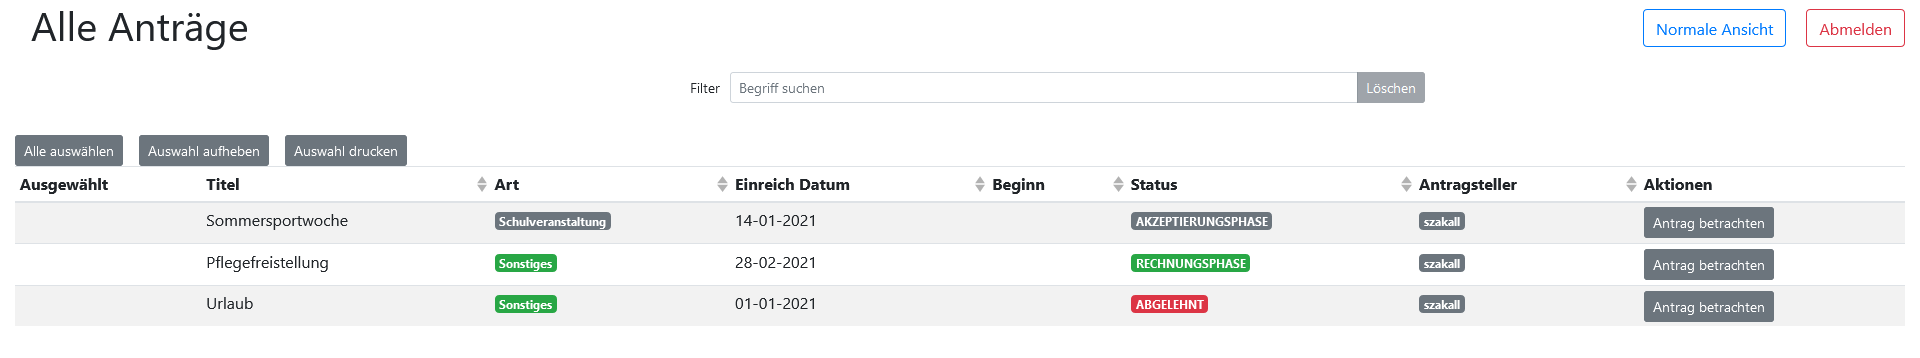
\includegraphics[width=1\linewidth]{images/website/admin}
	\caption[Aktiv]{Ein Bild der Admin Ansicht}
	\label{fig:adminview}
\end{figure}
Die farbig hinterlegten Elemente heißen \enquote{badges} und können wie folgt erstellt werden:
\begin{code}{html}
	<b-badge variant="danger">Rote Badge</b-badge>
	<b-badge variant="success">Grüne Badge</b-badge>
	<b-badge>Graue Badge</b-badge>
\end{code}
\captionof{listing}{Code - Badge Beispiel}
	\label{list:badgebsp} ~\\
~\\

\newpage
\paragraph{Administrator Antragsansicht}
~\\
Die Administrator Antragsansicht schaut gleich aus, wie die Ansicht der normalen Benutzer - mit einem Unterschied. Die Administratoren haben nicht die Funktionen \enquote{Speichern} und \enquote{Antrag schließen}, sondern \enquote{Antrag annehmen} und \enquote{Antrag ablehnen}. Falls der Antrag abgelehnt wird, taucht wieder eine Sicherheitsmeldung auf. Hier muss der Administrator eine Begründung, für die Ablehnung angeben. 
\begin{figure}[H]
	\centering
	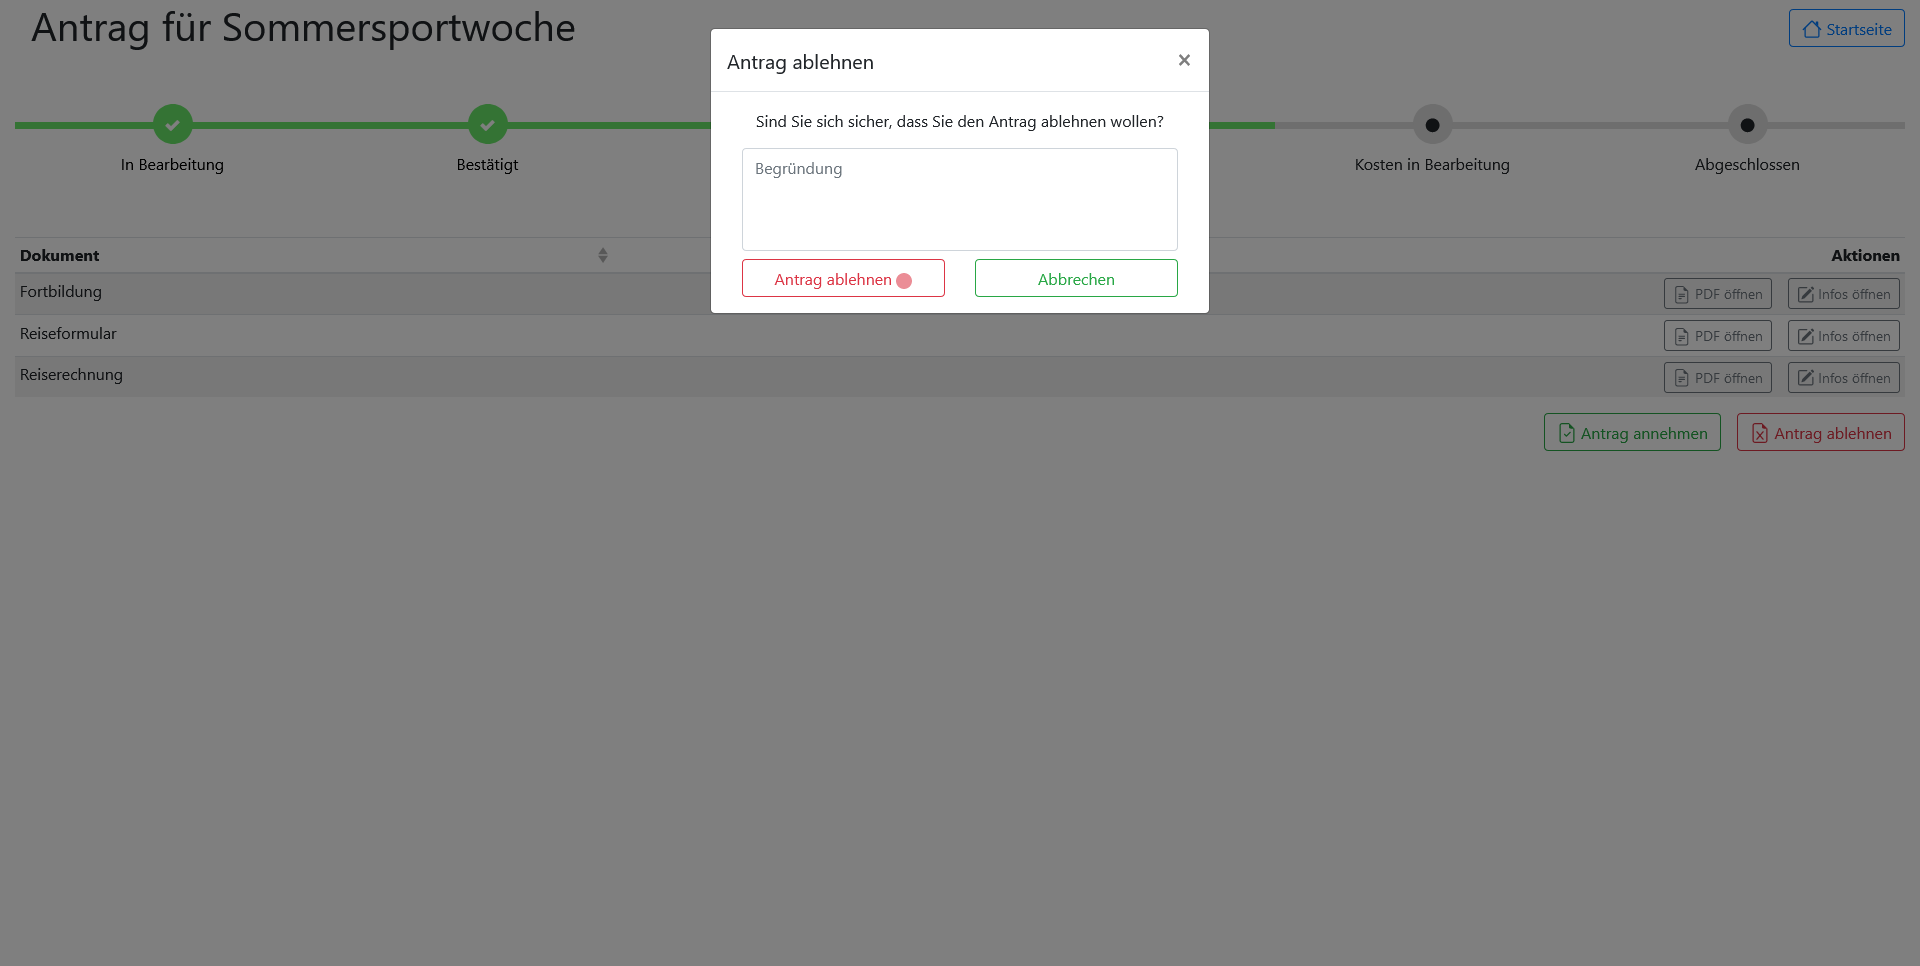
\includegraphics[width=0.6\linewidth]{images/website/admin_antrag_schiessen}
	\caption[Aktiv]{Ein Bild der Antrag ablehnen Meldung}
	\label{fig:adminclose}
\end{figure}
Im Code wird dieses Eingabefeld im \enquote{Modal} wie folgt erstellt:
\begin{code}{html}
	<!-- Antrag Ablehnen Warnhinweis -->
    <b-modal ref="close-modal" hide-footer title="Antrag ablehnen">
      <b-container fluid>
        <b-row
          ><b-col cols="12">
            <div class="d-block text-center">
              <p>
                Sind Sie sich sicher, dass Sie den Antrag ablehnen wollen?
              </p>
              <!-- Begründung der Ablehnung -->
              <b-form-textarea
                id="decline-reason"
                placeholder="Begründung"
                rows="3"
                no-resize
              ></b-form-textarea>
            </div> </b-col
        ></b-row>
        <b-row>
          <b-col cols="6">
            <!-- Antrag ablehnen Bestätigung -->
            <b-button class="mt-2" variant="outline-danger" block @click="delAn"
              >Antrag ablehnen <b-spinner small type="grow"></b-spinner
            ></b-button>
          </b-col>
          <b-col cols="6">
            <!-- Abbrechen Button -->
            <b-button
              class="mt-2"
              variant="outline-success"
              block
              @click="hideClose"
              >Abbrechen</b-button
            ></b-col
          >
        </b-row>
      </b-container>
    </b-modal>
\end{code}
\captionof{listing}{Code - Antrag ablehnen}
	\label{list:badgebsp} ~\\
\newpage
\subsubsection{Seite nicht Gefunden}
\label{chapter:implementierung-frontend-komponenten-notfound}
Falls der momentane Nutzer von \textit{Refundable} eine ungültige URL aufrufen möchte, wird dieser sofort informiert, dass er etwas falsch gemacht hat. Desweiteren wird dem Nutzer direkt eine Lösung vorgeschlaen, wie er dieses Problem beheben kann. Um dem Nutzer zu visualisieren, dass der \enquote{Website} Knopf die richtige Wahl ist, haben wir ihn in einem Grün hervorgehoben. Außerdem wird dem Aufrufer, der Seite mit schimmernden grauen Boxen, die einen \enquote{Lade-Zustand} visualisieren sollen gezeigt, dass die Seite, die der Nutzer aufrufen wollte nicht richtig lädt.
\begin{figure}[H]
	\centering
	
\includegraphics[width=1\linewidth]{images/website/notfound}
	\caption[Neuer Schulantrag]{Ein Bild der nicht Gefunden Seite}
	\label{fig:notfoundsite}
\end{figure}
~\\
Die Elemente, welche den Lade-Zustand verkörpern sollen, heißen \enquote{b-skeleton-img} und werden wie folgt erstellt:
\begin{code}{html}
	<b-skeleton-img animation="fade"></b-skeleton-img>
\end{code}
\captionof{listing}{Code - Skeleton}
	\label{list:codeskeleton} ~\\

\newpage
\subsubsection{Antrag suchen}
\label{chapter:implementierung-frontend-komponenten-suchen}
Um den Administratoren während ihren Tätigkeiten ein wenig Arbeit abzunehmen, wurde eine Möglichkeit eingebaut, einen Antrag direkt über eine Seite zu suchen. Dazu muss der Administrator die Unterseite \enquote{/viewer} aufrufen und kann, wie man in \autoref{fig:searchsite} sehen kann, die Antrags ID suchen und so direkt zu dem gewünschten Antrag gelangen.
\begin{figure}[H]
	\centering
	
\includegraphics[width=1\linewidth]{images/website/search}
	\caption[Neuer Schulantrag]{Ein Bild der Antrag suchen Seite}
	\label{fig:searchsite}
\end{figure}
~\\

\newpage 
\subsubsection{Rechte vergeben}
\label{chapter:implementierung-frontend-komponenten-rechte}
Während der Entwicklung ist uns aufgefallen, dass eine Funktion fehlt, einem bestimmten Benutzer mit gewissen Rechten auszustatten. Daher ist es dem \textit{Superuser} möglich über das Admindashboard Rechte zu vergeben. Dazu muss er nur die E-Mail Adresse des bestimmten Nutzers eingeben und mittels \textit{Radio-Buttons} die gewünschten Rechte auswählen. Auch hier wurden wieder die bekannten Elemente der restlichen Website verwendet.
\begin{figure}[H]
	\centering
	
\includegraphics[width=1\linewidth]{images/website/rechte}
	\caption[Neuer Schulantrag]{Ein Bild der Rechte vergeben Seite}
	\label{fig:rightssite}
\end{figure}